%\documentclass[12pt,twoside]{latex/memoireuqam1.3} % Pour version papier recto-verso
\documentclass[12pt]{latex/memoireuqam1.3}          % Pour version PDF


\usepackage[T1]{fontenc}
\usepackage[utf8]{inputenc} % Pour utiliser les caract�res Unicode, notaamment sous Linux

% fonts and lang packages
\usepackage[utf8]{inputenc} 	% utf8
\usepackage[T1]{fontenc} 	% french characters
\usepackage[french]{babel}	% french dictionnary

% utils
\usepackage{graphicx} 	% enhenced includes
\usepackage{latex/comment}	% comment blocks
\usepackage[hyphens]{url}		% display url links
\usepackage{rotating}	% rotating figues
%\usepackage{authblk}	% enhenced authors
\usepackage{color}		% colors
\usepackage{float}

\usepackage{tablefootnote}
\usepackage{ifthen}
\usepackage{tikz, tikz-qtree}

% tables
\usepackage{tabularx}
\usepackage{latex/multirow}

\usepackage{lmodern}
\usepackage{microtype}
\usepackage{natbib}

\usepackage{xcolor}
\usepackage[export]{adjustbox}
\definecolor{light-gray}{gray}{0.8}

% \usepackage{relsize}
\usepackage{subcaption}
\captionsetup[figure]{labelfont=bf}
\captionsetup[table]{labelfont=bf}

% renew authors
%\renewcommand\Authand{ et }
%\renewcommand\Authands{, et }

% listings
\usepackage{listings}

\lstset{
	inputencoding=utf8,
	basicstyle=\small\ttfamily,
	frame=none,
	numberstyle=\footnotesize,
	numbersep=5pt,
	tabsize=4,
	literate=
	{ç}{{\,c}}1
	{û}{{\^u}}1
	{é}{{\'e}}1
	{è}{{\`e}}1
	{ê}{{\^e}}1
	{à}{{\`a}}1
	{É}{{\'E}}1
	{È}{{\`E}}1
	{À}{{\`A}}1
	{`}{{\`{}}}1,
}

\usepackage{pdfpages}

\usepackage{nameref}
\usepackage{lscape}

% Change paragraph style
\usepackage{latex/titlesec}
\titleformat{\paragraph}[runin]
{\bfseries}{\theparagraph}{1em}{}

% maths packages
\usepackage{amsmath}
\usepackage{amssymb}
\usepackage{amsthm}

% Change asm questions styles
\makeatletter
\newtheoremstyle{indented}
  {3pt}% space before
  {3pt}% space after
  {\addtolength{\@totalleftmargin}{2.5em}
   \addtolength{\linewidth}{-2.5em}
   \parshape 1 2.5em \linewidth}% body font
  {}% indent
  {\bfseries}% header font
  { - }% punctuation
  {0em}% after theorem header
  {}% header specification (empty for default)
\def\th@plain{%
  \thm@notefont{}% same as heading font
  \itshape % body font
}
\def\th@definition{%
  \thm@notefont{}% same as heading font
  \normalfont % body font
}
\makeatother

\theoremstyle{indented}
\newtheorem{question}{Question}[section]
\newtheorem*{response}{Réponse}

\usepackage{latex/silence}
\WarningFilter{frenchb.ldf}{Figure}

% J'ai de la difficult\'e \`a lire quand les hyperliens sont vert
% pale. De plus, je crois que quand tu imprimeras les versions
% papier... cela risque de g\'en\'erer du texte plus pale, moins
% lisible... Donc j'ai desactive la couleur pour les liens... mais
% c'est facile de les reactiver: voir makefile.

\newboolean{ColoredLinks}
\setboolean{ColoredLinks}{true}


\usepackage[pdfborder={0 0 0}, colorlinks=true]{hyperref}
% compatibility between pdftex and hyperref
\ifthenelse{\boolean{ColoredLinks}}
{ \hypersetup{citecolor=blue} }
{ \hypersetup{colorlinks=false} }

\usepackage{wasysym}

%%%%%%%%%%%%%%%%%%%%%%%%%%%%%%%%%%%%%%%%%%%%%
%%%%%%%%%%%%%%% Macros et ajouts %%%%%%%%%%%%
%%%%%%%%%%%%%%%%%%%%%%%%%%%%%%%%%%%%%%%%%%%%%
\floatstyle{ruled}

\newfloat{programme}{htbp}{lop}[chapter]
\floatname{programme}{Programme}

\newcommand{\ACOMPLETER}[1]{{\textcolor{red}{#1}}}
\newcommand{\AVERIFIER}[1]{{\textcolor{blue}{#1}}}

\newcommand{\todo}[1]{{\textcolor{blue}{<\footnotesize A faire: #1>}}}
\newcommand{\TODO}[1]{{\textcolor{blue}{[[A FAIRE: #1]]}}}

\newcommand{\README}{{\sc readme}}
\newcommand{\DOCDOWN}{{\texttt{DocDown}}}
\newcommand{\MAN}{{\sc man}}

\newcommand\rot{\rotatebox{90}}

\newcommand{\Legende}[1]{{\footnotesize{\newline L\'egende: #1}}}

\newcommand{\B}{{$\bullet$}}

\newcommand{\subsectionSansNum}[1]{\paragraph{#1}{\ }}

% Pour presentation de sous-sections avec numero alphabetique
\newcounter{numSoussectionAlpha}
\setcounter{numSoussectionAlpha}{1}

\newcommand{\resetsoussectionAlpha}{\setcounter{numSoussectionAlpha}{1}}
\renewcommand{\thenumSoussectionAlpha}{\Alph{numSoussectionAlpha}}
\newcommand{\soussectionAlpha}[1]{\thenumSoussectionAlpha.~{\bf #1}{\ }\stepcounter{numSoussectionAlpha}}
\renewcommand{\soussectionAlpha}[1]{{\bf #1}{\ }\stepcounter{numSoussectionAlpha}}
%\renewcommand{\soussectionAlpha}[1]{{\bf #1}{\ }\stepcounter{numSoussectionAlpha}}

\newcommand{\captionEcosysteme}[1]{\caption[Place #1 dans l'\'ecosyst\`eme de documentation Nit.]{Place #1 dans l'\'ecosyst\`eme de documentation Nit.}}

\newcommand{\captionTaxonomieThemes}[1]{\caption[Taxonomie des
 th\`emes #1 les plus fréquents dans les fichiers \README.]{Taxonomie des
 th\`emes #1 les plus fréquents dans les fichiers \README.
 \Legende{\textbf{occ.}: nombre d'occurrences du thème dans le corpus;
 \textbf{\% occ.}: pourcentage d'occurrences associées à ce thème;
 \textbf{moy.}: moyenne du nombre d'occurrences du thème par document;
 \textbf{\# doc.}: nombre de documents contenant le thème;
 \textbf{\% doc.}: pourcentage de documents contenant le thème;
 \textbf{\% pos.}: position moyenne du thème dans les documents en pourcentage de la taille du document.
 Les thèmes sont triés par position moyenne dans les documents.}}}

\newcommand{\captionComparaisonExpert}[3]{\caption[Comparaison du
nombre #1 dans le fichier \README\ produit par l'expert~#2 pour la biblioth\`eque \texttt{#3}.]{Comparaison du
nombre #1 dans le fichier \README\ produit par l'expert~#2 pour la biblioth\`eque \texttt{#3} avec ceux issus de
GitHub analys\'es dans le chapitre~\ref{readmes-github} et ceux
\'ecrits par les experts Nit pour le corpus d'alignement du
chapitre~\ref{align}.}}

\newtheorem{definition}{D\'efinition}

% Items, and Enum
\newenvironment{Items}%
{\begingroup\setlength{\topsep}{.050\parsep}\addtolength{\parskip}{-.75\parskip}\setlength{\partopsep}{.25\partopsep}%
\begin{itemize}\setlength{\itemsep}{0pt}\addtolength{\parsep}{-.1\parsep}}%
{\end{itemize}\endgroup\smallbreak}

\newenvironment{Enum}%
{\begingroup\setlength{\topsep}{.050\parsep}\addtolength{\parskip}{-.75\parskip}\setlength{\partopsep}{.25\partopsep}%
\begin{enumerate}\setlength{\itemsep}{0pt}\addtolength{\parsep}{-.1\parsep}}%
{\end{enumerate}\endgroup\smallbreak}

\newcommand{\TT}[1]{{\tt #1}}

\floatstyle{boxed}
\newfloat{algorithme}{htbp}{lop}
\floatname{algorithme}{Algorithme}

\floatstyle{ruled}
\newfloat{pseudocode}{htbp}{lop}
\floatname{pseudocode}{Pseudocode}


\newcommand{\ppff}{\texttt{PpFf}}
\newcommand{\PpFf}{\ppff}

\newcommand{\GT}[1]{{{\textcolor{red}{\footnotesize [[(Guy T.) #1]]}}}}
\newcommand{\gt}[1]{}

\newcommand{\IC}[1]{{\textcolor{blue}{\footnotesize [[(Iulian C.) #1]]}}}
\newcommand{\ic}[1]{}

\lstset{
    language=C++,
    inputencoding=utf8,
    basicstyle=\small\ttfamily,
    frame=none,
    numberstyle=\footnotesize,
    numbersep=5pt,
    tabsize=4,
    literate=
    {?}{{\,c}}1
    {?}{{\^u}}1
    {?}{{\'e}}1
    {?}{{\`e}}1
    {?}{{\^e}}1
    {?}{{\`a}}1
    {?}{{\'E}}1
    {?}{{\`E}}1
    {?}{{\`A}}1
    {`}{{\`{}}}1,
}

\floatstyle{boxed}
\newfloat{Listing}{htbp}{lop}
\floatname{Listing}{Listing}

\newcommand{\M}[1]{\texttt{M#1}}
\newcommand{\Machine}[1]{\texttt{M#1}}

\newcommand{\graphe}[2]{\input{graphes/finaux/#1}}
\newcommand{\grapheref}[1]{\ref{#1.fig}}


\newcommand{\grapheH}[1]{\centering{\includegraphics[width=0.7\textwidth]{graphes/finaux/#1-here.png}\vspace*{-0.8cm}}}

\newcommand{\ExtraitTestUnitaire}{{\footnotesize~(Ce segment de code est un extrait d'un test unitaire. Les d\'etails exacts de l'assertion ont \'et\'e omis.)}}


% Ajouts par Iulian
% \usepackage{booktabs}	% Pour utiliser ent�te du tableau (commande \midrule)
\usepackage{longtable} % Pour utiliser les tables sur plusieurs pages
\usepackage[paper=portrait,pagesize]{typearea}
% \usepackage{natbib}
\setcounter{secnumdepth}{3} % Pour subsubsectionz
\usepackage{tikz} % Pour cr�er des graphiques
\usepackage{pgfplots} % Pour cr�er des graphiques


\usepackage{framed}
\usepackage{nameref}


\begin{document}

%%%%%%%%%%%%%%%%%%%%%%%%%%%%%%%%%%%%%%%%%%%%%
%%%%%%%%%%%%%%% Page de titre %%%%%%%%%%%%%%%
%%%%%%%%%%%%%%%%%%%%%%%%%%%%%%%%%%%%%%%%%%%%%

\title{TRAITEMENT EFFICACE DE FLUX DE DONN\'EES SUR MACHINES MULTI-C\OE{}URS \`A L'AIDE DE FASTFLOW}

\title{\emph{P\lowercase{p}F\lowercase{f}}~: Une API C++ pour le traitement parall\`ele de flux de donn\'ees}

\author{Iulian Ciobanu}
\degreemonth{D\'ecembre}
\degreeyear{2019}
\uqammemoire
\matiere{informatique}

\thispagestyle{empty}
\maketitle

%%%%%%%%%%%%%%%%%%%%
% Page préliminaires
%%%%%%%%%%%%%%%%%%%%

% D'apres le guide, c'est BIBLIOGRAPHIE qu'il faut utiliser, et c'est ce qui est defini aussi par le template!
\renewcommand \bibname{BIBLIOGRAPHIE}

\renewcommand \listfigurename{LISTE DES FIGURES}
\renewcommand \listtablename{LISTE DES TABLEAUX}
\renewcommand \lstlistlistingname{LISTE DES LISTINGS}
\renewcommand \appendixname{ANNEXE}
\renewcommand \figurename{Figure}
\renewcommand \tablename{Tableau}

\pagenumbering{roman}
\addtocounter{page}{1}

%%%%%%%%%%%%%%%%%%%%%%%%%%%%%%%%%%%%%%%%%%%%%
%%%%%%%%%%%%%%% Remerciements %%%%%%%%%%%%%%%
%%%%%%%%%%%%%%%%%%%%%%%%%%%%%%%%%%%%%%%%%%%%%


   \parskip=0pt
   \vspace*{0.1 truecm} 
   \begin{center}
    {\uppercase { REMERCIEMENTS }}\par
   \end{center}
   \nobreak \vspace*{1.10 truecm}
   \parskip=2ex



Tout grand accomplissement est rarement r\'ealis\'e par une seule personne. Celle-ci ne fait pas exception. Je suis reconnaissant \`a tous ceux qui m'ont aid\'e et soutenu pendant ces ann\'ees de travail.

Tout d'abord, je voudrais remercier \`a mon superviseur, le professeur Guy Tremblay. Sans son soutien et son aide, cette th\`ese n'aurait pas pu \^etre termin\'ee. Gr\^ace \`a sa riche exp\`erience, il m'a guid\'e dans mes recherches. Il m'a donn\'e de nombreuses id\'ees, suggestions et critiques de valeur.

Je dois \'egalement un grand merci au professeur Marco Aldinucci pour tout son soutien technique pour l'application de \TT{FastFlow}. 

Je souhaite remercier les ing\'enieurs du syst\`eme des laboratoires informatiques et le personnel administratif  qui ont permis \`a ma th\`ese de se d\'erouler sans obstacle technique ou administratif.

Enfin, je tiens \`a remercier \`a ma famille, qui a toujours \'et\'e l\`a, de m'aider moralement \`a surmonter les difficult\'es que j'ai eues en toutes ces ann\'ees de recherches. 




%%%%%%%%%%%%%%%%%%%%%%%%%%%%%%%%%%%%%%%%%%%%%
%%%%%%%%%%%%%%%%%%%% TOC %%%%%%%%%%%%%%%%%%%%
%%%%%%%%%%%%%%%%%%%%%%%%%%%%%%%%%%%%%%%%%%%%%

\setcounter{tocdepth}{2}

\tableofcontents
\listoffigures
\listoftables

\lstlistoflistings
\addtocontents{toc}{\protect\vspace{1.5ex}}
\addcontentsline{toc}{chapter}{\UpperRef{LISTE DES LISTINGS}}

%%%%%%%%%%%%%%%%%%%%%%%%%%%%%%%%%%%%%%%%%%%%%
%%%%%%%%%%%%%%%%% Résumé %%%%%%%%%%%%%%%%%%%%
%%%%%%%%%%%%%%%%%%%%%%%%%%%%%%%%%%%%%%%%%%%%%

\begin{abstract}

Les logiciels classiques de traitement de donn\'ees sont b\^atis sur le concept de persistance o\`u les donn\'ees, pr\'ealablement stock\'ees, sont interrog\'ees et mise \`a jour plusieurs fois tout au long de leur dur\'ee de vie. Cependant, pour plusieurs applications, les donn\'ees arrivent de fa\c con continue, \`a grande vitesse, et elles doivent \^etre trait\'ees de fa\c con incr\'ementale sans la possibilit\'e de faire plusieurs passages sur les donn\'ees. La complexit\'e de ces types d'applications augmente encore plus lorsque les donn\'ees sont trait\'ees en parall\`ele. Afin de traiter de fa\c con simple et efficace les flux de donn\'ees, ce m\`emoire propose un \TT{API} de haut niveau dans le langage \TT{C++}. En utilisant la biblioth\`eque \TT{FastFlow}, l'interface permet aux utilisateurs d'exposer facilement le parall\'elisme dans des applications s\'equentielles.
	
	
\end{abstract}



%%%%%%%%%%%%%%%%%%%%%%%%%%%%%%%%%%%%%%%%%%%%%
%%%%%%%%%%%%%% Introduction %%%%%%%%%%%%%%%%%
%%%%%%%%%%%%%%%%%%%%%%%%%%%%%%%%%%%%%%%%%%%%%

\begin{introduction}


%\GT{L'introduction n'est pas un chapitre num\'erot\'e.}

\label{introduction.chap}

Blah blah \ldots

Signalons que l'utilisation du package \TT{inputenc} permet d'utiliser
des caractères accentués normaux, plutôt que des caractères accentués
dans l'ancien style (commandes pour les accents).\footnote{Le même
texte écrit avec les accents en commande serait alors le suivant~:
<<Signalons que l'utilisation du package \TT{fontenc} permet
d'utiliser des caract\`eres accentu\'es normaux, plut\^ot que des
caract\`eres accentu\'es dans l'ancien style (commandes pour les
accents).>>}

On remarquera aussi, dans la note en bas de page, l'utilisation des
guillemets français, appelés aussi parfois des <<chevrons>>, qu'on
doit utiliser plutôt que les ``guillemets anglais''.  Ces guillemets
français s'obtiennent à l'aide des caractères
\TT{<}\TT{<}\ldots\TT{>}\TT{>}.

Une autre façon est de définir la macro suivante, puisqu'avec certains
\emph{packages}, les caract\`eres \TT{<}\TT{<}\ldots\TT{>}\TT{>} ne
semblent pas fonctionner~:
{\small
\begin{verbatim}
  \newcommand{\QUOTE}[1]{\og #1 \fg{}}
\end{verbatim}
} 


\newpage

blah blah blah

\end{introduction}



%%%%%%%%%%%%%%%%%%%%%%%%%%%%%%%%%%%%%%%%%%%%%
%%%%%%%%%%%%%%%%%%% Main %%%%%%%%%%%%%%%%%%%%
%%%%%%%%%%%%%%%%%%%%%%%%%%%%%%%%%%%%%%%%%%%%%


\chapter{Langages existants de traitement de flux de donn\'ees~: \TT{Spark}, \TT{Java} et \TT{FastFlow}}
\label{outils_connus}
\label{outils_connus.chap}

\gt{Un nouveau chapitre doit (habituellement) avoir quelques
paragraphes d'introduction, qui indiquent ce dont va traiter le
chapitre.  Ce peut \^etre quelques paragraphes pr\'esent\'es
directement, sans num\'ero de section.  Ce peut aussi \^etre, quand il
y a plusieurs \'el\'ements \`a pr\'esenter, une section .1 appel\'ee
Introduction.  Ici, quelques paragraphes, sans section, devraient
\^etre suffisants.}


\ic{J'ai ajout\'e une petite introduction pour ce chapitre.}



\gt{Concernant les citations~: il y a deux macros que tu peux
utiliser: cite vs.\ citep: tu dois utiliser cite si tu veux que les
noms d'auteurs apparaissent comme sujet dans une phrase (avec
l'ann\'ee entre parenth\`eses)~; tu dois utiliser citep si tu veux que
la r\'ef\'erence soit compl\`etement entre parenth\`eses. Voir les
exemples ci-haut et ci-bas.}


La programmation parall\`ele devient de plus en plus une n\'ecessit\'e avec l'apparition des architectures multicœurs. Jusqu'\`a il y a quelques ann\'ees, une des principales fa\c{c}ons d'ex\'ecuter un programme plus rapidement \'etait gr\^ace \`a l'augmentation de la vitesse d'horloge du processeur. De nos jours, la vitesse d'horloge a atteint ses limites et les performances d'un programme ne peuvent souvent \^etre am\'elior\'ees que si on l'ex\'ecute en parall\`ele. 

Il existe de nombreuses approches et de nombreux langages de programmation parall\`ele.
%
Le paradigme de programmation parall\`ele \emph{par flux de donn\'ees} offre une approche prometteuse pour la programmation de syst\`emes multicœurs. C'est cette approche que nous allons bri\`evement d\'ecrire avant de pr\'esenter trois langages existants qui mettent en \oe{}uvre cette approche.

\section{Parall\'elisme de flux de donn\'ees}


Les flux de donn\'ees sont utilis\'es dans plusieurs domaines, par exemple, traitement d'images, de donn\'ees r\'eseau, de donn\'ees et transactions boursi\`eres, de donn\'ees de trafic routier, etc.

\GT{Ici, il faudrait dire quelques mots rapides sur ce qu'est le
traitement par flux de donn\'ees --- m\^eme si tu l'as d\'ej\`a
mentionn\'e dans l'introduction --- pour que ce soit plus
complet/coh\'erent!}

\GT{C'est aussi ici, il me semble, qu'il serait bien d'expliquer la
diff\'erence entre les applications qui traitent de grandes
quantit\'es de donn\'ees par lots (en \emph{batch}, \emph{offline}),
alors que d'autres les traitent en ligne (\emph{online}), de fa\c{c}on
incr\'ementale, au fur et \`a mesure o\`u ces donn\'ees deviennent
disponibles.}



Il existe de nombreux syst\`emes de traitement de flux de donn\'ees. La conception, le mod\`ele et l'architecture de ces syst\`emes diff\`erent, de sorte qu'ils poss\`edent des fonctionnalit\'es et des performances diff\'erentes. Ce chapitre pr\'esente un aper\c{c}u de trois syst\`emes de traitement de flux de donn\'ees~: \TT{Apache Spark} (Sect.~\ref{spark.sect}), les \TT{Stream}s de \TT{Java}~8 (Sect.~\ref{java8.sect}) et \TT{FastFlow} (Sect.~\ref{fastflow.sect}).  Ce sont trois parmi les nombreux syst\`emes actuellement disponibles, que nous avons choisis de pr\'esenter parce qu'ils ont servi d'inspiration et de base au syst\`eme que nous avons d\'evelopp\'e, \ppff, que nous pr\'esenterons aux chapitres~\ref{description.chap} et~\ref{implementation.chap}.


\section{Apache Spark}

\label{spark.sect}

\gt{Ci-bas~: Si tu dis que Spark est pour r\'esoudre certaines
probl\'ematiques de MapReduce, il faudrait que tu mentionnes
bri\`evement quelles sont ces probl\'ematiques. Il faudrait aussi ---
est-ce le cas? --- que la r\'ef\'erence porte sur ces
probl\'ematiques, pas sur MapReduce en g\'en\'eral, donc Hadoop est
simplement une mise en oeuvre.}

\ic{J'ai reformul\'e la description de Spark}


\TT{Apache Spark}~\citep{apachSpark} est un engin de traitement de flux de donn\'ees dot\'e d'une API expressive qui permet aux d\'eveloppeurs d'ex\'ecuter efficacement plusieurs op\'erations sur une collection de donn\'ees. \TT{Spark} est un outil de traitement par lots, mais qui a aussi des capacit\'es de traitement de flux incr\'emental de donn\'ees. Il se concentre principalement sur l'acc\'el\'eration du traitement des donn\'ees en gardant en m\'emoire les donn\'ees de travail, ce qui permet notamment l'acc\'el\'eration du traitement des algorithmes it\'eratifs.

Alors que le traitement en m\'emoire contribue consid\'erablement \`a obtenir de hautes performances, Spark est \'egalement rapide avec le traitement de donn\'ees sur disques en raison de l'optimisation qui peut \^etre r\'ealis\'ee en analysant l'ensemble complet des t\^aches \`a l'avance. Ceci peut \^etre r\'ealis\'e en cr\'eant des graphes acycliques dirig\'es (DAG) qui repr\'esentent toutes les op\'erations qui doivent \^etre ex\'ecut\'ees, les donn\'ees \`a \^etre utilis\'ees, ainsi que les relations entre elles. \`A l'aide de ce graphe, le syst\`eme d'ex\'ecution a la capacit\'e de planifier et d'ordonnancer le travail de fa\c{c}on efficace.

\TT{Spark} utilise un mod\`ele appel\'e \emph{Resilient Distributed Datasets} (\TT{RDD})~\citep{Salloum2016} pour repr\'esenter les collections de donn\'ees, mod\`ele qui g\`ere efficacement la persistence lorsque les donn\'ees ne peuvent pas toutes \^etre trait\'ees en m\'emoire ou lorsqu'elles doivent \^etre pr\'eserv\'ees pour \'eviter des recalculs. De plus, \TT{Spark} impl\'emente le mod\`ele \emph{Discretized Streams}~\citep{zaharia2013discretized} pour le traitement de flux incr\'emental de donn\'ees.
%
Nous expliquons ces deux mod\`eles dans les sous-sections qui suivent.


\subsection{\emph{Resilient Distributed Dataset} (\TT{RDD})}

Un \TT{RDD} est une abstraction de donn\'ees en m\'emoire qui \'evite la r\'eplication de donn\'ees et minimise les acc\`es au disque. L'utilisation de \TT{RDD}s permet aux applications de mettre en cache des donn\'ees \`a travers diff\'erentes \'etapes de traitement, ce qui acc\'el\`ere consid\'erablement la r\'eutilisation pour les traitements futurs. De plus, les \TT{RDD}s m\'emorisent les op\'erations utilis\'ees pour les construire et utilisent un m\'ecanisme de \emph{checkpoint}. Lorsqu'une panne survient, les \TT{RDD}s requis peuvent \^etre reconstruits, et ce sans devoir tout refaire les calculs.

Les \TT{RDD}s sont conçus pour \^etre partitionn\'es, donc r\'epartis sur diff\'erentes machines. Chaque partition contient des enregistrements qui peuvent \^etre cr\'e\'es par op\'erations de transformations. Les transformations incluent notamment les opérations \TT{map}, \TT{filter}, \TT{groupBy} et \TT{join}.


\GT{Je crois que le paragaphe qui suit est redondant par rapport \`a
ce qui est \'ecrit plus haut, non? C'est-\`a-dire qu'il redit la
m\^eme chose...}

Les \TT{RDD}s peuvent \^etre cr\'e\'es via d'autres \TT{RDD}s existants. Ce m\'ecanisme permet la reconstruction des partitions perdues, car chaque \TT{RDD} dispose d'informations suffisantes sur la reconstruction \`a partir d'autres \TT{RDD}s. Lorsqu'il y a une demande de mise en cache d'un \TT{RDD}, par d\'efaut \TT{Spark} stocke ces partitions en m\'emoire. Cependant, des partitions peuvent aussi \^etre stock\'ees sur disques, lorsque la m\'emoire est insuffisante.


\subsection{\emph{Discretized Streams}}

\TT{Spark} traite un flux incr\'emental de donn\'ee par l'implémentation du mod\`ele \emph{Discretized Streams} (\TT{D-stream}s).   
%
\GT{Je ne comprends pas la phrase qui suit.}
%
Les \TT{D-stream}s repr\'esentent les flux de donn\'ees re\c{c}us en entr\'ee pour un traitement. 
%
TT{Spark} d\'ecompose un flux de donn\'ees en une s\'erie de lots, en fonction de courts intervalles de temps, lots appel\'es \emph{micro-batches}. Chaque \emph{micro-batch} stocke ses donn\'ees dans un \TT{RDD}. Ensuite, la \emph{micro-batch} est trait\'ee et ses r\'esultats sont stock\'es dans des \TT{RDD}s interm\'ediaires.


\subsection{Exemple~: \TT{wordCount}}


\begin{lstlisting}[
basicstyle=\footnotesize\tt,
label={wordCountSpark},
language=java,
caption={Un segment de code \TT{Spark/Java} pour compter le nombre d'occurrences de mots. Exemple provenant du site Web pour \TT{Apache Spark} (\url{https://spark.apache.org/examples.html}).},
frame=single,
escapechar=\#,
float]
JavaRDD<String> textFile = 
    sc
    .textFile("hdfs://...");

JavaPairRDD<String, Integer> counts = 
    textFile
    .flatMap( s -> Arrays.asList(s.split(" ")).iterator() )
    .mapToPair( word -> new Tuple2<>(word, 1) )
    .reduceByKey( (a, b) -> a + b );

counts
    .saveAsTextFile("hdfs://...");
\end{lstlisting}


Afin d'illustrer le mod\`ele de programmation avec les \TT{RDD}s de \TT{Spark}, le listing~\ref{wordCountSpark} montre le code source d'un segment de code d\'ecompte des mots, code \'ecrit en \TT{Java}.%
%
\footnote{\url{https://spark.apache.org/examples.html}}
%
Plus pr\'ecis\'ement, ce segment de code compte le nombre d'occurrences des divers mots dans un fichier texte et compos\'e de plusieurs op\'erations~: 
\begin{itemize}
\item Blah, blah
\end{itemize}



\section{\TT{Stream}s de \TT{Java} 8}
\label{java8.sect}

La version 8 de \TT{Java}, qui a introduit les \TT{Stream}s, a chang\'e la façon dont les d\'eveloppeurs peuvent traiter, tant de fa\c{c}on s\'equentielle que parall\`ele, les collections de donn\'ees. La manipulation de collections de donn\'ees \`a l'aide de \TT{Stream}s ressemble \`a un langage de requ\^etes de base de donn\'ees. Au lieu de parcourir explicitement les donn\'ees \`a l'aide de boucles (\TT{for}), un d\'eveloppeur sp\'ecifie simplement une suite d'op\'erations \emph{fonctionnelles} \`a effectuer sur les \'el\'ements d'une collection. \cite{urma2014java} fournissent une description d\'etaill\'ee des nouveaux concepts introduits dans \TT{Java~8}. Les \TT{Stream}s et les \emph{expressions lambdas} sont les fonctionnalit\'es les plus remarquables ajout\'ees dans l'API \citep{javaStreamAPI}. Ils sont con\c{c}us pour traiter les collections de donn\'ees de mani\`ere simple et efficace. Les sous-sections qui suivent d\'ecrivent quelques-uns des concepts de \TT{Java~8}.


\subsection{Expressions lambda}


\gt{Bon, apr\`es avoir jet\'e un coup d'oeil \`a la documentation de
lstlisting et \`a des m\'emoires et th\`eses r\'ecentes, je constate
qu'il est pr\'ef\'erable {\bf de ne pas utiliser la macro Listing},
mais d'utiliser plut\^ot les divers arguments de l'environnement
lstlisting.  Ceci permettra une pr\'esentation plus uniforme des
diff\'erents listings et, surtout, une num\'erotation correcte (et
uniforme), dans le vrai style requis~: listing 1.1, 1.2, etc. pour le
chapitre 1; listing 2.2, 2.2, etc pour la chapitre 2 --- donc comme
pour les figures.}


\begin{lstlisting}[
label={exLambda},
language=java,
gobble=4,
caption={[Un exemple d'une expression lambda qui re\c{c}oit deux valeurs de type entier en argument.]Un exemple d'une expression lambda qui re\c{c}oit deux valeurs de type entier en argument, affect\'ee \`a la variable \TT{a}. Un appel est ensuite effectu\'e et le r\'esultat est affect\'e \`a la variable \TT{result}.},
frame=single,
float]
    interface Addable { int add (int x, int y); }
    
    int x = 3;
    int y = 2;
    
    // Affectation de l'expression lambda a une variable.
    Addable a = (int w, int z) -> { return w + z; };

    // Appel de l'expression lambda.
    int result = a.add(x, y);    
\end{lstlisting}



Une \emph{expression lambda} ---  appel\'ee aussi \emph{fonction anonyme} --- est un bloc de code avec des param\`etres qui peut \^etre d\'efini, comme n'importe quelle valeur, puis qui peut \^etre ex\'ecut\'e ult\'erieurement. Par exemple, la fonction anonyme du listing~\ref{exLambda}, qui re\c{c}oit deux valeurs de type entier en argument et renvoie leur somme, est affect\'ee \`a la variable \TT{a}. Un appel \`a la m\'ethode \TT{add} --- de l'interface \TT{Addable} --- est ensuite effectu\'e avec des arguments effectifs (\TT{x} et \TT{y}).


\begin{lstlisting}[
label={lambdaAsFonctionalInterface},
language=java,
gobble=4,
caption={Remplacement d'une classe anonyme avec une expression lambda.},
frame=single,
float]
    // Specification d'un thread avec une classe interne anonyme.
	Thread th = new Thread( new Runnable() {
		public void run() {
          ... // Code a executer par le thread.
		}
	});

    // Specification d'un thread avec une expression lambda.
	Thread th = new Thread( () -> {
         ... // Code a executer par le thread.
	});
\end{lstlisting}


\gt{Citation trop r\'ecente pour Haskell, qui ne montre pas que c'est quand m\^eme un ancien langage. Je l'ai remplac\'e. Idem pour Lisp.}

Le concept d'expression lambda n'est pas nouveau. Il est utilis\'e depuis longtemps dans les langages de programmation fonctionnelle tels que \TT{Lisp}~\citep{Steele84} ou \TT{Haskell}~\citep{HudakWad90,hutton2016programming}.
%
Les expressions lambda rendent le code plus concis et, dans le cas de \TT{Java}, l'\'etendent avec des concepts de langages de programmation fonctionnelle. 

Plus sp\'ecifiquement, en \TT{Java}, ce concept est li\'e \`a celui d'interface fonctionnelle. Une expression lambda peut \^etre sp\'ecifi\'ee \`a la place d'une valeur dont le type est une interface fonctionnelle. Par exemple, le listing~\ref{lambdaAsFonctionalInterface} montre un exemple o\`u un \TT{Thread th}, d\'eclar\'e en utilisant la syntaxe de classe anonyme, peut \^etre \'ecrit plus facilement avec une expression lambda.

Dans une expression lambda, lors de la compilation, les types des arguments peuvent \^etre automatiquement d\'etermin\'es par le compilateur. Cette fonctionnalit\'e permet de passer des m\'ethodes comme arguments plut\^ot que de construire un objet d'une classe sp\'ecifique. Ceci permet \`a un programmeur de construire facilement des pipelines d'op\'erations fonctionnelles.


\subsection{It\'erations}


\begin{lstlisting}[
label={comparisonInternVsExtern},
language=java,
gobble=4,
caption={[Comparaison entre une it\'eration externe et interne.]Une comparaison entre une it\'eration externe et interne. Dans le cas de l'it\'eration externe, le d\'eveloppeur d\'efinit une boucle explicite pour traiter les divers \'el\'ements de la collection.  Le traitement appliqu\'e \`a chaque \'el\'ement consiste \`a convertir la cha\^ine en lettres majuscules si elle d\'ebute par la lettre <<\TT{J}>>. Le m\^eme traitement est appliqu\'e dans le cas de l'it\'eration interne. Par contre, dans ce cas, c'est le \TT{Stream} --- produit par l'appel <<\TT{myList.stream()}>> --- qui contr\^ole le processus d'it\'eration~; l'usager  indique simplement les diverses op\'erations \`a effectuer, en les chainant les unes \`a la suite des autres.},
frame=single,
float]
    List<String> myList =
            Arrays.asList("Tom", "John", "Harry", "Jonathan");

    // Iteration externe avec ajout explicite (style imperatif).
    List<String> resultExtern = new ArrayList<String>();
    for (String s: myList){
        if (s.startsWith("J")) // Selection
           // Transformation et ajout dans le resultat.
           resultExtern.add(s.toUpperCase()); 
    }
        
    // Iteration interne avec pipeline d'operations (style fonctionnel).
    List<String> resultIntern = 
        myList
        .stream()
        .filter(s -> s.startsWith("J")) // Selection.
        .map(String::toUpperCase)       // Transformation.
        .collect(Collectors.toList());  // Collecte du resultat.
\end{lstlisting}


Une it\'eration est le processus qui consiste \`a traverser une collection d'\'el\'ements pour traiter chacun d'entre eux. Avec les \TT{Stream}s \TT{Java}, une it\'eration peut \^etre ex\'ecut\'ee de deux mani\`eres : par une it\'eration \emph{externe} ou \emph{interne}. 

Une it\'eration est dite \emph{externe} lorsque le d\'eveloppeur contr\^ole la travers\'ee des \'el\'ements.  L'acc\`es et l'op\'eration sur chaque \'el\'ement de la collection sont d\'efinis par l'utilisateur. Par contre, une it\'eration est dite \emph{interne} lorsque la collection contr\^ole elle-m\^eme tous les d\'etails du processus d'it\'eration. L'utilisateur fournit uniquement les op\'erations permettant de traiter les \'el\'ements, sans se soucier de la mani\`ere dont les \'el\'ements sont acc\'ed\'es et fournis. Le listing~\ref{comparisonInternVsExtern} montre un exemple d’une comparaison entre une itération externe et interne. 

L'approche interne est attrayante pour les opportunit\'es qu'elle offre aux compilateurs, notamment l'optimisation de l'exécution et les m\'ecanismes de nettoyage n\'ecessaires en arri\`ere-plan. Un autre avantage des it\'erations internes est l'efficacit\'e, le traitement pouvant \^etre r\'eparti entre les cœurs de la machine pour une ex\'ecution parall\`ele.


\begin{figure}
\centering
     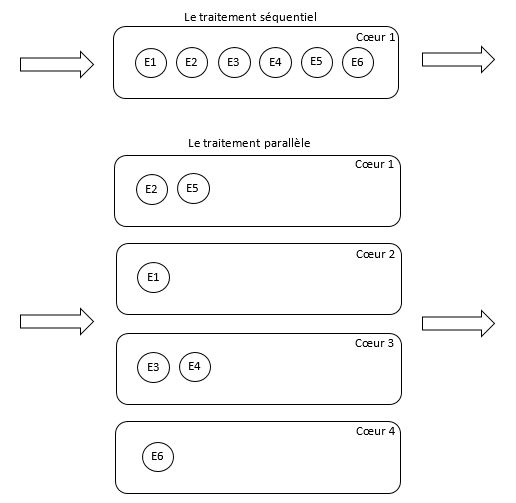
\includegraphics[width=1.0\textwidth]{Figures/ComparisonSequentialVsParallel.jpg}
      \caption[Une comparaison entre traitement s\'equentiel et parall\`ele.]{Une comparaison entre traitement s\'equentiel et parall\`ele. Les six \'el\'ements du flux (\TT{E1}, \ldots,  \TT{E6}) sont r\'epartis dans quatre sous-flux. Chaque sous-flux est trait\'e par l'un de quatre cœurs disponibles. Les r\'esultats sont combin\'es apr\`es le traitement.}
       \label{ComparisonSequentialVsParallel.fig}
\end{figure}


Lorsqu'un flux s'ex\'ecute en parall\`ele, \TT{Java} partitionne le flux en plusieurs sous-flux. Les op\'erations parcourent et traitent ces sous-flux en parall\`ele, puis combinent les r\'esultats. La figure~\ref{ComparisonSequentialVsParallel.fig} montre la comparaison entre  un traitement s\'equentiel et un traitement parall\`ele, dans cet exemple avec quatre c\oe{}urs. Les \'el\'ements du flux sont partitionn\'es en sous-flux et chaque sous-flux r\'esultant est trait\'e par l'un de quatre cœurs disponibles.  



\subsection{Flux}


\begin{lstlisting}[
label={findFirst},
language=java,
gobble=2,
caption={Optimisation du traitement d'un flux en utilisant la technique d'\'evaluation court-circuit\'ee.},
frame=single,
float]
	List<Employee> employees;
	Optional<Employee> employee = employees.findFirst();
\end{lstlisting}


Un flux est d\'efini comme une s\'equence immuable d'\'el\'ements fournissant une vari\'et\'e d'op\'erateurs et de m\'ethodes permettant de traiter une collection de donn\'ees. Le flux prend en charge les op\'erations d'agr\'egation \citep{javaStreamAggregate} s\'equentielles et parall\`eles sans se soucier de la mani\`ere dont les \'el\'ements sont stock\'es ou accessibles. Pour effectuer un traitement, les op\'erations de flux sont compos\'ees dans un \TT{pipeline}. Un \TT{pipeline} est compos\'e d'une source, de z\'ero ou plusieurs op\'erations interm\'ediaires et d'une op\'eration terminale. Une source peut \^etre constitu\'ee d'une collection ou de tout objet impl\'ementant l'interface qui d\'efinit le m\'ecanisme permettant d'extraire les donn\'ees de la source. 
Les op\'erations sur les flux adoptent un m\'ecanisme d'\'evaluation paresseuse. L'\'evaluation paresseuse est une m\'ethode d'optimisation du traitement qui retarde l'\'etape du calcul jusqu'\`a ce que le r\'esultat soit nécessaire. En \TT{Java}, le traitement sur les \'el\'ements du flux est r\'ealis\'e seulement \`a l'activation de l'op\'eration finale et les \'el\'ements source ne sont consomm\'es qu'au besoin. Cela permet au compilateur d'optimiser le traitement des donn\'ees dans le \TT{pipeline}.
Une autre technique d'optimisation utilis\'ee par \TT{Java} est l'\'evaluation court-circuit\'ee (\emph{short-circuiting} en anglais). Dans un flux, une telle \'evaluation a pour effet que seuls les \'el\'ements n\'ecessaires sont consomm\'es.%
%
\footnote{L'\'evaluation court-circuit\'ee peut aussi \^etre vue comme une forme d'\'evaluation paresseuse, bien que la documentation \TT{Java} distingue ces deux formes d'optimisation.}
%
Par exemple, dans le listing~\ref{findFirst}, l'opérateur \TT{findFirst} retourne le premier employ\'e trouv\'e dans une liste d'employ\'es~; les \'el\'ements restants du flux sont ignor\'es.


L'un des principaux avantages des flux est qu'ils peuvent \^etre \'evalu\'es soit de fa\c{c}on s\'equentielle, soit en parall\`ele. L'\'evaluation s\'equentielle est r\'ealis\'ee en ex\'ecutant toutes les op\'erations en \TT{pipeline} sur chaque \'el\'ement du flux. Lorsqu'un flux est \'evalu\'e en parall\`ele, il utilise un type sp\'ecial d'it\'erateur appel\'e \TT{Spliterator}. Ce dernier partitionne le flux de mani\`ere r\'ecursive en se divisant lui-m\^eme pour cr\'eer des flux enfants. Ce m\'ecanisme permet aux \emph{threads} de traverser plusieurs flux en parall\`ele. Les \emph{threads} sont g\'er\'es par un groupe de \emph{threads} de type \TT{fork/join}.


\subsection{\emph{Threads} de type \TT{fork/join}}

Introduit en \TT{Java~7}, le \emph{framework} \TT{fork/join} permet aux d\'eveloppeurs de sp\'ecifier des t\^aches pouvant \^etre subdivis\'ees et ex\'ecut\'ees en parall\`ele sur des machines multicœurs. Il est bas\'e sur deux op\'erations : \TT{fork} et \TT{join}. L'op\'eration \TT{fork} a pour r\^ole de diviser une t\^ache en plus petites sous-t\^aches ind\'ependantes, et ce  r\'ecursivement jusqu'\`a ce qu'elles soient assez simples pour \^etre ex\'ecut\'ees de mani\`ere ind\'ependante et asynchrone. L'op\'eration \TT{join} a pour r\^ole de fusionner les r\'esultats de toutes les sous-t\^aches de mani\`ere r\'ecursive en un seul r\'esultat.
Les sous-t\^aches obtenues par l'op\'eration \TT{fork} sont soumises \`a un \TT{ForkJoinPool}. Ce dernier est composé d'un ensemble de travailleurs. Le nombre de travailleurs dans un \TT{ForkJoinPool} est g\'en\'eralement limit\'e par le nombre de cœurs de la machine. Chaque travailleur peut ex\'ecuter une t\^ache \`a la fois. Les t\^aches en attente d'ex\'ecution sont stock\'ees dans une file appartenant \`a un travailleur. Une t\^ache en cours d'ex\'ecution peut g\'en\'erer de nouvelles t\^aches, qui sont ensuite mises en file  pour une ex\'ecution ult\'erieure. Lorsqu'un travailleur a termin\'e l'ex\'ecution d'une t\^ache, il essaie de prendre une t\^ache des files des autres travailleurs \`a l'aide d'un algorithme de vol de travail (\emph{work stealing algorithm}~\cite{FrigoLeiRan98}). Cet algorithme permet un \'equilibrage efficace de la charge de travail entre les divers travailleurs.


\subsection{Exemple~: \TT{wordCount}}


\begin{lstlisting}[
basicstyle=\footnotesize\tt,
label={wordCountJava},
language=java,
caption={Un pipeline \TT{Java} pour compter le nombre d'occurrences de mots.},
frame=single,
escapechar=\#,
float]
public static void main(String[] args) throws IOException {
  // Le texte a analyser, sous forme d'une chaine.
  String text = "Lorem ipsum dolor sit amet, consectetur \n" +
                " adipiscing elit. Lorem ipsum dolor sit amet, consectetur \n" +
                " adipiscing elit. Lorem ipsum dolor sit amet.";

  // Le texte a analyser decompose en une liste de lignes.
  ArrayList<String> lines = 
	new ArrayList<String>(Arrays.asList(text.split("\\n")));

  // Le pipeline qui traite la liste de lignes.	
  List<Map.Entry<String,Integer>> wordsCount = 
    lines
    .stream()
    .parallel()
    .flatMap(line->Arrays.stream(line.trim().split(" ")))
    .map(word->word.replaceAll("[^a-zA-Z]", "").toLowerCase())
    .filter(word->word.length() > 0)
    .map(word->new SimpleEntry<>(word, 1))
    .collect(toMap(e->e.getKey(), e->e.getValue(), (v1,v2)->v1+v2))
    .entrySet()
    .stream()
    .collect(Collectors.toList());   	
  
  wordsCount.forEach( x -> System.out.println("'" + x.getKey() + 
                                              "' => " + x.getValue()) );
}
#\vspace{-1cm}#
#\hrule#
#\underline{R\'esultat de l'ex\'ecution:}#
  'dolor' => 3
  'lorem' => 3
  'amet' => 3
  'adipiscing' => 2
  'ipsum' => 3
  'elit' => 2
  'consectetur' => 2
  'sit' => 3
\end{lstlisting}


\GT{Ci-bas: j'ai chang\'e des d\'etails des explications car ce n'est
pas une application compl\`ete et \c{c}a traite pas un fichier texte
mais juste une chaine.}


Afin d'illustrer le mod\`ele de programmation avec les \TT{Stream}s de \TT{Java~8}, le listing~\ref{wordCountJava} montre le code source d'un segment de code \TT{Java} de d\'ecompte de mots. Plus pr\'ecis\'ement, ce segment de code compte le nombre d'occurrences des mots dans un chaine et est compos\'ee de plusieurs op\'erations \emph{cha\^in\'ees} les unes \`a la suite des autres :

\begin{itemize}
	\item \TT{Files.lines}, qui renvoie un flux s\'equentiel de lignes \`a partir du fichier. Le fichier est rep\'er\'e par le param\`etre \TT{inputFile} fourni en argument.

\GT{Tu utilises \TT{lines} qui est un \TT{ArrayList}, donc tu
n'utilises par \TT{File.lines}! De plus, tu as aussi l'appel \`a
\TT{stream}, donc tu ne parles pas.  Mais est-il vraiment
n\'ecessaire, si c'est ensuite suivi de \TT{parallel}? \`A
v\'erifier!}

	\item \TT{parallel}, qui marque le flux en tant que flux parall\`ele. Cette op\'eration permet ainsi de partitionner et d'ex\'ecuter le \TT{pipeline} en parall\`ele.

	\item \TT{flatMap}, qui divise chaque ligne en mots qui sont ensuite transmis en aval sous forme d'\'el\'ements de donn\'ees individuels.
	
	\item \TT{map}, qui supprime tous les caract\`eres qui ne sont pas des lettres puis transforme les lettres majuscules du mot en minuscules.
	
	\item \TT{filter},  s\'electionne dans le flux seulement les mots qui ne sont pas vides.
	
	\item \TT{map}, qui cr\'ee une paire (de type \TT{Entry}) avec une cl\'e repr\'esent\'ee par le mot et une valeur associ\'ee \'egale \`a 1.
	
	\item \TT{collect},  collecte les \'el\'ements dans un \TT{Map} et additionne le nombre d'occurrences de chacun des mots \`a l'aide de l'expression lambda.
	
	\item \TT{entrySet},  renvoie un flux de type cl\'e--valeur. La cl\'e est le mot et la valeur est son nombre d'occurrences dans le fichier.

	\item \TT{stream}, cr\'ee un nouveau flux de donn\'ees \`a partir de l'ensemble de paires.
	
	\item Finalement \TT{collect}, qui combine tous les \'el\'ements dans une liste.
	
	
\end{itemize}


\section{\TT{FastFlow}}
\label{fastflow.sect}

\TT{FastFlow} est une biblioth\`eque \TT{C++} qui, \`a la base, offre un ensemble de m\'ecanismes de bas niveau pour traiter les flux de donn\'ees et s'ex\'ecutant sur des machines multicœurs avec m\'emoire partag\'ee. La facilit\'e de d\'eveloppement avec \TT{FastFlow} est rendue possible en utilisant un ensemble de \emph{squelettes algorithmiques} offerts par la biblioth\`eque~\citep{AldinucciEtAl14}. Son efficacit\'e provient principalement de la mise en œuvre optimis\'ee de m\'ecanismes de communication de bas niveau et de sa conception en couches. Les squelettes algorithmiques offerts par \TT{FastFlow} peuvent \^etre utilis\'es pour exprimer les mod\`eles les plus courants de parall\'elisme. Ces squelettes algorithmiques peuvent \^etre imbriqu\'es pour cr\'eer des mod\`eles hi\'erarchiques de parall\'elisme plus complexes.

\TT{FastFlow} a \'et\'e conçue selon plusieurs principes: conception en couches, efficacit\'e des communications et synchronisation, et support pour le parall\'elisme de flux.

\subsection{Conception en couches}

\begin{figure}
\centering
     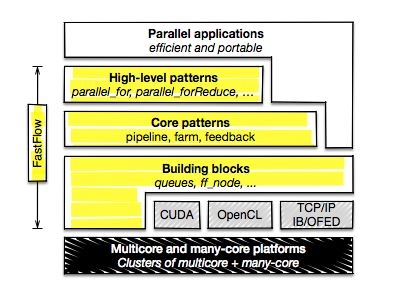
\includegraphics[width=1.0\textwidth]{Figures/FastFlowLayers.jpg}
      \caption[Les couches de \TT{FastFlow}.]{Les couches de \TT{FastFlow} --- figure tir\'ee de~\citep{Torquati15}.}
       \label{FastFlowLayers.fig}
\end{figure}


\TT{FastFlow} a \'et\'e conçue sous la forme d'une pile de couches pour permettre d'impl\'ementer des m\'ecanismes d'abstraction et d'optimisation \`a plusieurs niveaux. La figure~\ref{FastFlowLayers.fig} montre les trois principales couches: \emph{High-level patterns}, \emph{Core patterns} et \emph{Building blocks}. 

Le niveau le plus bas de la pile, \emph{Building blocks}, g\`ere les communications asynchrones entre les canaux de communication et g\`ere le cycle de vie des flux. Plus pr\'ecis\'ement, cette couche offre des services pour les couches sup\'erieures. Elle g\`ere les queues, les processeurs et les fils d'ex\'ecutions (\emph{threads}).

Au-dessus de la couche \emph{Building blocks} se trouve la couche \emph{Core patterns}, qui fournit des squelettes (gabarits) pour mod\'eliser diff\'erentes formes de parall\'elisme de flux. Les trois mod\`eles fournis dans cette couche sont \emph{task-farm}, \emph{pipeline} et \emph{feedback}, qui permettent de construire des flux parall\`eles vari\'es. 

Au sommet de la pile se trouve la couche \emph{High-level patterns}, qui permet d'exprimer le parall\'elisme de plus haut niveau. Elle fournit plusieurs m\'ethodes qui couvrent les paradigmes de programmation parall\`eles les plus courants : parall\'elisme de flux, parall\'elisme de donn\'ees et  parall\'elisme de t\^aches. 

\subsection{Efficacit\'e}

L'id\'ee de \TT{FastFlow} est de fournir au programmeur des files (\emph{queues}) \emph{MP (Multiple Producer)} et des files \emph{MC (Multiple Consumer)} sans verrouillage, et ce afin de supporter des acc\`es rapides aux flux de donn\'ees. G\'en\'eralement, dans les applications de flux de donn\'ees, les canaux de communication sont impl\'ementés via des files de type \emph{MPMC (Multiple Producer/Multiple Consumer)}. Dans ce modèle, les acteurs se synchronisent simultanément pour acc\'eder aux donn\'ees. Ces synchronisations sont habituellement support\'ees par une ou plusieurs op\'erations atomiques --- par exemple, \TT{Compare-And-Swap} --- qui se comportent comme des barri\`eres de m\'emoire, ce qui augmente le co\^ut des synchronisations. Afin d'\'eviter les barri\`eres de m\'emoire, \TT{FastFlow} b\^atit les files \emph{MPMC} en assemblant des files, sans barri\`ere de m\'emoire, de type \emph{SPSC (Single Producer/Single Consumer)}. Dans ce mod\`ele, des files d’ex\'ecution regroupent ou \'emettent les donn\'ees des files d'entr\'ee vers les files de sortie. Selon son r\^ole, une file d'ex\'ecution peut \^etre un \TT{Emitter} ou un \TT{Collector}. Alors que l'\TT{Emitter} lit les donn\'ees, le \TT{Collector} \'ecrit sur une ou plusieurs files de types \emph{SPSC}. Contrairement aux op\'erations atomiques, ce m\'ecanisme n\'ecessite seulement des copies de m\'emoire --- la performance offerte par cette solution d\'ecoule de la vitesse sup\'erieure de la copie par rapport \`a la barri\`ere de m\'emoire.


\subsection{Parall\'elisme de flux}

Dans \TT{FastFlow}, le parall\'elisme de flux est repr\'esent\'e par un flux de donn\'ees comportant une s\'erie d'\'etapes, s\'equentielles ou parall\`eles, appel\'ees \emph{stages}. Chaque \emph{stage} lit les donn\'ees \`a partir du flux d'entr\'ee, effectue des calculs et traitements, puis \'ecrit le r\'esultat sur le flux de sortie. Le calcul repr\'esente une s\'equence de transformations sur les donn\'ees. Le parall\'elisme est obtenu en ex\'ecutant chaque \emph{stage} simultan\'ement sur des \'el\'ements ind\'ependants ou sur des sous-s\'equences d'\'el\'ements. 

Dans \TT{FastFlow}, le parall\'elisme peut \^etre obtenu en exploitant directement les mod\`eles parall\`eles disponibles dans la couche \emph{Building blocks}. En particulier, cela peut \^etre r\'ealis\'e des deux fa\c{c}ons suivantes :

\begin{itemize}
\item en d\'efinissant des activit\'es concurrentes s\'equentielles en sous-classant la classe \TT{ff\_node}~;
 
\item en construisant des mod\`eles parall\`eles complexes en composant de mani\`ere hi\'erarchique des activit\'es concurrentes s\'equentielles, soit avec des \emph{pipelines} --- \TT{ff\_pipeline} --- ou des \emph{farms} --- \TT{ff\_farm}.
\end{itemize}

\subsubsection*{La classe \TT{ff\_node}}

Dans \TT{FastFlow}, \TT{ff\_node} est la classe de base pour un noeud de traitement. Elle fournit les m\'ecanismes appropri\'es pour d\'efinir des activit\'es s\'equentielles pour le traitement de données apparaissant sur un canal d'entr\'ee et fournissant les r\'esultats correspondants sur un canal de sortie. 

\goodbreak
\begin{samepage}
La classe \TT{ff\_node} d\'efinit plusieurs m\'ethodes, les trois plus importantes \'etant les suivantes :
\begin{lstlisting}[language=c++]
    virtual void* svc(void* task) = 0
    virtual int svc_init() { return 0; } 
    virtual void svc_end() {} 
\end{lstlisting}
\end{samepage}

La premi\`ere m\'ethode, \TT{svc} (mn\'emonique <<service>>), est la plus importante car c'est celle qui d\'efinit le comportement du nœud lors du traitement des \'el\'ements du flux d'entr\'ee. Quant aux deux autres m\'ethodes, elles sont appel\'ees lorsque le traitement repr\'esent\'e par le nœud est d\'emarr\'e \TT{(svc\_init)} et juste avant qu'il soit termin\'e \TT{(svc\_end)}. Ces trois m\'ethodes virtuelles peuvent \^etre red\'efinies dans des sous-classes \TT{ff\_node} sp\'ecifi\'ees par le programmeur afin d'impl\'ementer le traitement, l'initialisation ou la finalisation du code.


\subsubsection*{La classe \TT{ff\_pipeline}}

Un \emph{pipeline} est utilis\'e pour mod\'eliser les traitements exprim\'es par des \emph{stages}. Il est repr\'esent\'e par la classe \TT{ff\_pipeline}. Un {pipeline} peut comporter plusieurs \emph{stages}, peut \^etre construit comme un pipeline \`a \emph{n} \emph{stages}, ou encore comme un {pipeline} de {pipelines}. Un \emph{stage} peut \^etre de type \TT{ff\_node} ou \TT{ff\_farm}.


\goodbreak

\subsubsection*{La classe \TT{ff\_farm}}
\label{farm.sect}

\begin{figure}[htbp]
     \centering
     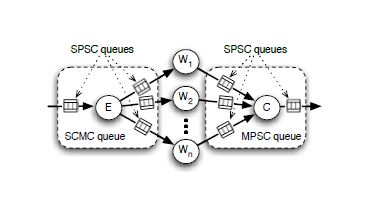
\includegraphics[width=1.0\textwidth]{Figures/FastFlowFarm.jpg}
      \caption[Les trois parties d'un \emph{farm} de \TT{FastFlow}.]{Un \emph{farm} de \TT{FastFlow} est compos\'e de trois parties~:  l'\TT{Emitter (E)}, le \emph{pool} de \TT{workers} (W1\ldots\ Wn) et le \TT{Collector (C)}. Les canaux de communication sont impl\'ement\'es en assemblant des files de types \emph{Simple Producer/Simple Consumer (SPSC)} --- figure tir\'ee de~\citep{aldinucci2010efficient}.}
       \label{FastFlowFarm.fig}
\end{figure}

Un \emph{farm} est bas\'e sur la r\'eplication d'une fonction. Dans \TT{FastFlow}, un \emph{farm} est repr\'esent\'e par un objet de la classe \TT{ff\_farm}. Comme le montre la figure~\ref{FastFlowFarm.fig}, un \emph{farm} est compos\'e de trois parties distinctes: un \TT{Emitter}, un  \emph{pool} de \TT{workers} et un \TT{Collector}. L'\TT{Emitter} est responsable de la r\'epartition des \'el\'ements du flux au \emph{pool} de \TT{workers}, lesquels traitent et produisent les donn\'ees de sortie; l'\TT{Emitter} distribue les \'el\'ements d'entr\'ee aux travailleurs selon une certaine politique d'ordonnancement afin d'\'equilibrer la charge des travailleurs. Les r\'esultats sont ensuite rassembl\'es par le \TT{Collector} dans un seul flux de sortie. Les communications entre \TT{Emitter} et \TT{Collector} se font via des canaux de communication sans barri\`eres de m\'emoire, tel que d\'ecrit pr\'ec\'edemment.


\subsection{Exemple~: \TT{WordCount}}


\begin{lstlisting}[language=c++, 
caption={Le code source \TT{FastFlow} d'une application pour compter le nombre d'occurrences de mots.},
label={wordcountFastFlow},
frame=single,
float,
numbers=left
]
 #define DEFAULT_INPUT_FILE "Words.txt"
 typedef std::vector<std::string> Words;
 
 struct linesFromFileStage: ff_node {
    std::string const &path;
    linesFromFileStage(std::string const &path): path(path){}
 
    void* svc(void* task) {
       std::ifstream file(path);
       std::string* line = new std::string;
       while (std::getline(file, *line)) {
           ff_send_out(line);
           line = new std::string;
       }
       return EOS;
    }
 };
 
 struct splitInWordsStage: ff_node {
    std::string delimiter = " ";
    void* svc(void* task) {
       std::string line = *((std::string*)task);
       Words* words = new Words();
       size_t start = 0, end = 0;
       do {
           end = line.find(delimiter, start);
           size_t len = end - start;
           words->push_back( line.substr(start, len) );
           start += len + delimiter.length();
       } while (end != std::string::npos);

       return words;
    }
 };
\end{lstlisting}
 
\begin{lstlisting}[language=c++, frame=single,float,numbers=left,firstnumber=35]
 struct flatStage: ff_node {
    std::string delimiter = " ";
    void* svc(void* task) {
        for (auto &elem: *(Words*)task) {
            ff_send_out(&elem);
        }
        return GO_ON;
    }
 };
 
 struct groupByKeyStage: ff_node {
    typedef std::unordered_map<std::string, int> CONTAINER;
    CONTAINER &container;
    groupByKeyStage(CONTAINER &container): container(container){}
    void* svc(void* task) {
       container[*((std::string*)task)] += 1;
       return GO_ON;
    }
 };
\end{lstlisting}
 
\begin{lstlisting}[language=c++, frame=single, float, numbers=left,firstnumber=54]
 int main(int argc, char *argv[]) {
     std::unordered_map<std::string, int> result;
     std::string inputFile = DEFAULT_INPUT_FILE;

     if (argc >= 2) { inputFile = argv[1]; } 

     linesFromFileStage linesFromFile(inputFile);
     splitInWordsStage splitInWords;
     flatStage flat;
     groupByKeyStage groupByKey(result);

     ff_pipeline ffp;
     ffp.add_stage(&linesFromFile);
     ffp.add_stage(&splitInWords);
     ffp.add_stage(&flat);
     ffp.add_stage(&groupByKey);

     if (ffp.run_and_wait_end() < 0) error("running pipe");
     return 0;
 }
\end{lstlisting}

Cette section pr\'esente un exemple d'un programme r\'ealis\'e en \TT{FastFlow}. Illustr\'e dans le listing~\ref{wordcountFastFlow}, ce programme compte le nombre d'occurrences des divers mots dans un fichier texte. 

Un {pipeline} de \TT{n} \TT{stages} distincts est cr\'e\'e en instanciant les \TT{n} diff\'erents \TT{stages}; ensuite leurs r\'ef\'erences sont transmises dans le bon ordre au {pipeline}. Dans l'exemple du listing~\ref{wordcountFastFlow}, les \TT{stages} sont repr\'esent\'es par les op\'erations du programme de d\'ecompte du nombre de mots --- lignes 66 \`a 69.  Les quatre op\'erations r\'ealisent les fonctions suivantes :

\begin{itemize}
    \item \TT{linesFromFile}, qui renvoie un flux s\'equentiel de lignes \`a partir du fichier. Le fichier est identifi\'e par le param\`etre \TT{inputFile} fourni en argument.

    \item \TT{splitInWords}, qui divise chaque ligne en mots qui sont ensuite transmis en aval sous forme d'une collection de mots.
    
    \item \TT{flat}, qui décompose la collection en mots individuels, lesquels sont ensuite transmis dans le flux en tant qu'éléments individuels de données.
    
    \item \TT{groupByKey}, qui regroupe les mots similaires ensemble et ensuite compte le nombre d'occurrences de chaque mot.
    
\end{itemize}



\chapter{Description de l'API de \PpFf}
\label{description.chap}

\gt{Pour \'eviter la confusion, tu dois utiliser les m\^emes termes
que dans l'API, m\^eme si ces termes sont en anglais. Mais tu les mets
dans la police courrier, avec texttt.}

Ce chapitre pr\'esente l'API de \ppff. Sa conception permet aux utilisateurs de tirer parti de la simplicit\'e d'utilisation tout en cachant la complexit\'e concernant les m\'ecanismes concurrents utilis\'es. La figure~\ref{ComponentsAPI.fig} pr\'esente une vue d'ensemble de l'architecture du syst\`eme. L'API est compos\'ee de quatre \'el\'ements principaux: l'Interface avec laquelle le d\'eveloppeur interagit, les \texttt{Pipeline}s --- qui sont le coeur de l'API ---, les \texttt{Stage}s et les \texttt{Operator}s. Le r\^ole de chaque composant dans l'API est pr\'esent\'e dans la section suivante. La derni\`ere section  d\'ecrit plus en d\'etail les principales m\'ethodes de l'interface.



\begin{figure}[ht]
\centering
     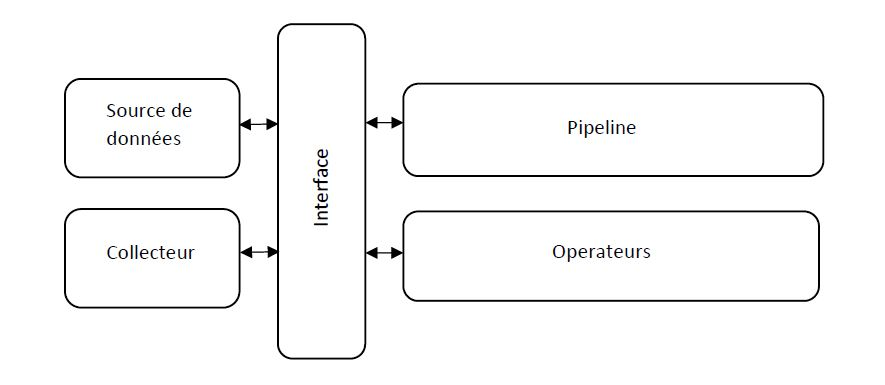
\includegraphics[width=1.0\textwidth]{Figures/ComponentsAPI.jpg}
      \caption{Composants de l'API de \ppff.}
       \label{ComponentsAPI.fig}
\end{figure}


\section{Les composants de l'API de \ppff}

L'\texttt{API} de \texttt{PpFf} est impl\'ement\'e au-dessus de la biblioth\`eque \texttt{FastFlow}. Les mod\`eles \texttt{Pipeline} et \texttt{Farm} fournis par cette biblioth\`eque sont utilis\'es comme bloc de construction pour rendre les fonctionnalit\'es de notre \texttt{API}. Cette section d\'ecrit le r\^ole de chaque composant de \texttt{PpFf} et leur mappage aux mod\`eles de \texttt{FastFlow}. La figure~\ref{fig:ClassDiagramme} pr\'esente une vue d'ensemble des classes qui compose l'\texttt{API}. 

\begin{figure}[ht]
\centering
     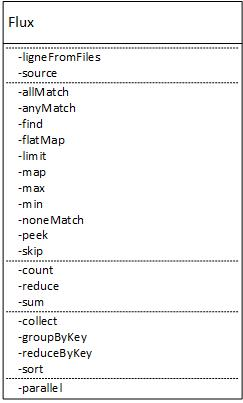
\includegraphics[width=1.0\textwidth]{Figures/ClassDiagramme.jpg}
      \caption{Les classes qui compose l'\texttt{API}.}
       \label{fig:ClassDiagramme}
\end{figure}
%
%\GT{Probablement qu'un diagramme de classe UML serait int\'eressant et
%utile.  Il pourrait \^etre introduit ici, puis expliqu\'e dans les
%sous-sections qui suivent.}
%
%\GT{Note que de fa\c{c}on g\'en\'erale, lorsqu'on d\'ebute une section
%qui contient plusieurs sous-sections, il est pr\'ef\'erable d'avoir
%quelques lignes d'introduction, qui donnent une vue d'ensemble de ce
%qui suit. Pas toujours, mais ici, avec le diagramme de classes, \c{c}a
%ferait l'affaire.}
%
%\IC{Mon plan initial \'etait de d\'ecrire les composants dans le chapitre 2 (Description de l'API de PpFf) et de pr\'esenter la partie technique dans le chapitre 3 (Impl\'ementation). Dans la premi\`ere partie du chapitre 2 j'ai choisi de d\'ecrire les composants principaux de l'API et dans la deuxi\`eme partie de ce chapitre de pr\'esenter quelques m\'ethodes avec des exemples. 
%Dans le chapitre 3 j'ai eu l'intention d'introduire un diagramme de classe UML en expliquant les classes qui compose l'API. } 
%
%\IC{Qu'est-ce que vous en pensez ? Est-ce que je dois introduire le diagramme dans le chapitre 2 ? Je ne suis pas sûr que je fasse la différence entre la description et implémentation de l’API.
%}


%\GT{La description est tout ce qu'un programmeur doit savoir/connaitre
%pour \underline{utiliser} ton API --- de l'ext\'erieur, comme une
%boite noire. L'impl\'ementation d\'ecrit les <<d\'etails>>
%n\'ecessaires pour comprendre \underline{comment fonctionne} l'API,
%par exemple, ce qu'un mainteneur devrait comprendre/connaitre s'il
%voulait modifier, corriger ou \'etendre ton API.}
%
%\GT{En lien avec le diagramme de classes, si l'utilisateur de l'API
%utilise ou manipule diff\'erents concepts et classes dans son
%programme, que ces concepts/classes sont utiles pour pouvoir utiliser
%correctement l'API --- avec la bonne syntaxe et la bonne s\'emantique
%--- alors ces concepts devraient \^etre d\'ecrits, par un diagramme de
%classes par exemple.}

\subsection{Interface}

L'interface propos\'ee en PpFf consiste en un ensemble de m\'ethodes qui permettent \`a l'utilisateur de manipuler des flux de donn\'ees de mani\`ere simple et efficace. L'interface suit d'assez pr\`es celle introduite pour les \emph{Streams} de Java~8. Le tableau~\ref{methodes_api.tab} d\'ecrit bri\`evement les m\'ethodes impl\'ement\'ees dans l'API.




%\GT{Dans un tabular, pour mettre du texte, on utilise p avec une
%largeur. Ceci \'evite de mettre des sauts de lignes explicites, ce qui
%n'est jamais une bonne id\'ee.}

%\GT{Il faut mettre le code avec police tt. Par contre, j'ai essay\'e
%que le code soit mis par d\'efaut ainsi, mais cela n'a pas
%fonctionn\'e, d'o\`u les commandes tt ins\'er\'ees en d\'ebut de
%chaque ligne~:(}
%
%\GT{Par contre, le d\'efaut avec la solution actuelle, c'est que c'est
%tr\`es difficile \`a comprendre pour les m\'ethodes plus complexes. Il
%faudra qu'on r\'efl\'echisse \`a une fa\c{c}on plus claire de
%pr\'esenter la signaure des m\'ethodes.}
%
%\IC{J'ai ajout\'e toutes les m\'ethodes d\'efinies dans l'interface de l'API dans ce tableau et j'ai \'et\'e oblig\'e d'utiliser le paquet longtable parce qu'elle s'\'etendait sur plusieurs pages. J'ai essay\'e de pr\'esenter la signature des m\'ethodes dans un format plus concis. Par exemple le paramètre std ::fonction a \'et\'e remplac\'e pour Func; j'ai enlev\'e les mots typename de chaque d\'eclaration de template; le param\`etre <typename ELEM, class ALLOC = std ::allocator<ELEM class TContainer >> a \'et\'e remplac\'e pour Container. De plus je n'ai pas pu r\'eutiliser la fonction qui redimensionne le tableau resizebox(textwidth). J'ai utilis\'e une police de caract\`ere plus petite (tiny) pour pouvoir encadrer le tableau dans la page.
%}
%
%\IC{J'ai reformul\'e la description pour le r\'esultat de la fonction flatMap}


%\begin{landscape}
\newpage
\KOMAoptions{paper=landscape,pagesize}
\recalctypearea


\begin{center}
\footnotesize
\begin{longtable}{|l|l|p{5cm}|}
\caption{Les m\'ethodes expos\'ees aux utilisateurs par l'API de~\ppff.\label{methodes_api.tab}}\\
\hline
\textbf{M\'ethode} & \textbf{Type du r\'esultat} & \textbf{Description du r\'esultat}\\
\hline
\endfirsthead
\multicolumn{3}{c}%
{\tablename\ \thetable\ (\textit{suite})} \\
\hline
\textbf{M\'ethode} & \textbf{Type du r\'esultat} & \textbf{Description du r\'esultat}\\
\hline
\endhead
\hline \multicolumn{3}{r}{\textit{Suite page suivante}} \\
\endfoot
\hline
\endlastfoot
\hline
	\begin{tabular}{@{}l@{}}
	\tt template<T> \\
	\tt allMatch(Func<bool(T*)> predicate)
	\end{tabular} &
  	\texttt{bool} &
    Retourne \texttt{true} si tous les \'el\'ements
    du flux satisfont \texttt{predicate}, sinon \texttt{false}.
    \\
\hline
	\begin{tabular}{@{}l@{}}
	\tt template<T> \\
	\tt anyMatch(Func<bool(T*)> predicate)
	\end{tabular} &
  	\texttt{bool} & 
    Retourne \texttt{true} si au moins un  
    \'el\'ement du flux satisfait \texttt{predicate}, sinon \texttt{false}.
\\
\hline
	\begin{tabular}{@{}l@{}}
	\tt template<T, Container<T>{>}\\
	\tt collect()
	\end{tabular} &
  	\texttt{Container<T>} &
    Retourne un conteneur
    STL avec tous les \'el\'ements du flux.
    \\
\hline
	\begin{tabular}{@{}l@{}}
	\tt count()\\
	\end{tabular} &
  	\texttt{unsigned int} & 
    Retourne le nombre d'\'el\'ements
    du flux.
    \\
\hline
	\begin{tabular}{@{}l@{}}
	\tt template<In> \\
	\tt find(Func<bool(In*)> const\& predicate)
	\end{tabular} &
  	\texttt{Pipe\&} &
    Retourne les
    \'el\'ements du flux qui satisfont \texttt{predicate}.
    \\
\hline
	\begin{tabular}{@{}l@{}}
	\tt template<In, Out, Container> \\
	\tt flatMap(Func<Container*(In*)> const\& taskFunc)
	\end{tabular} &
  	\texttt{Pipe\&} & 
    Applique la fonction fournie en argument
    \`a chaque \'el\'ement du flux et concat\`ene ces \'el\'ements lorsque plusieurs sont produits par la fonction.
    \\
\hline
	\begin{tabular}{@{}l@{}}
	\tt template<In, Out, Container=In> \\
	\tt flatMap()
	\end{tabular} &
  	\texttt{Pipe\&} &
    Produit un flux avec les \'el\'ements du conteneur.  
    \\
\hline
	\begin{tabular}{@{}l@{}}
	\tt template<In, K=In, V=In, MapType> \\
	\tt groupByKey(Func<K*(In*)> fk, Func<V*(In*)> fv)
	\end{tabular} &
  	\texttt{MapType} &
    Retourne un dictionnaire (\emph{map}) avec les \'el\'ements
    du flux regroupés par cl\'e.
   \\
\hline
%	\begin{tabular}{@{}l@{}}
%	\tt template<T, Container> \\
%	\tt intermediateCollect()
%	\end{tabular} &
%	\texttt{Collection<T, Container>} &
%    Retourne une collection avec les
%    \'el\'ements du flux. \GT{Est-ce utile de mentionner cette m\'ethode?}
%    \\ 
%\hline
	\begin{tabular}{@{}l@{}}
	\tt template<T> \\
	\tt limit(int n)
	\end{tabular} &
	\texttt{Pipe\&} & 
    Retourne un flux compos\'e des \texttt{n}~premiers \'el\'ements du flux d'entr\'ee.
    \\
\hline
	\begin{tabular}{@{}l@{}}
	\tt linesFromFile(string\& path)
	\end{tabular} &
	\texttt{Pipe\&} & 
    Retourne un flux avec les lignes
    contenues dans le fichier indiqu\'e par \texttt{path}.
    \\
\hline
	\begin{tabular}{@{}l@{}}
	\tt template<In, Out> \\
	\tt map(Func<Out*(In*)> const\& taskFunc)
	\end{tabular} &
	\texttt{Pipe\&} & 
    Retourne un flux compos\'e de
    l'application de \texttt{taskFunc}
    \`a chacun des
    \'el\'ements du flux.
    \\
\hline
	\begin{tabular}{@{}l@{}}
	\tt template<T> \\
	\tt max(Func<void(T*, T*)> compare)
	\end{tabular} &
	\texttt{T} &
	Retourne l'\'el\'ement maximum du flux en fonction du comparateur.
    \\
\hline
	\begin{tabular}{@{}l@{}}
	\tt template<T> \\
	\tt min(Func<void(T*, T*)> compare)
	\end{tabular} &
	\texttt{T} &
	Retourne l'\'el\'ement minimum du flux en fonction du comparateur.
    \\
\hline
	\begin{tabular}{@{}l@{}}
	\tt template<T> \\
	\tt noneMatch(Func<bool(T*)> predicate)
	\end{tabular} &
	\texttt{bool} &
    Retourne \texttt{true} si aucun des \'el\'ements
    du flux ne satisfait \texttt{predicate},
    sinon \texttt{false}.
    \\
\hline
	\begin{tabular}{@{}l@{}}
	\tt parallel(int workers = 1)
	\end{tabular} &
	\texttt{Pipe\&} &
	Sp\'ecifie le nombre de travailleurs \`a utiliser pour traiter les \'el\'ements du flux.
    \\
\hline
	\begin{tabular}{@{}l@{}}
	\tt template<In> \\
	\tt peek(Func<void(In*)> const\& taskFunc)
	\end{tabular} &
	\texttt{Pipe\&} &
	Applique la fonction \texttt{taskFunc} \`a chaque \'el\'ement du flux et r\'e\'emet l'\'el\'ement (sans le modifier) sur le flux de sortie. Note: Utile pour le d\'ebogage.
    \\
\hline
	\begin{tabular}{@{}l@{}}
	\tt template<In, Out=In> \\
	\tt reduce(Reducer<In, Out> const\& reducer)
	\end{tabular} &
	\texttt{Out} &
	Effectue une r\'eduction sur les \'el\'ements du flux. Voir la notion de \texttt{reducer}, p.~\pageref{reducer.sect}.
    \\
\hline
	\begin{tabular}{@{}l@{}}
	\tt template<In, Out=In> \\
	\tt reduce(Out init, Func<Out(In, Out)> acc)
	\end{tabular} &
	\texttt{Out} &
	Effectue une r\'eduction des \'el\'ements du flux, en utilisant \texttt{init} comme valeur initiale et \texttt{acc} comme fonction d'accumulation.
    \\
\hline
	\begin{tabular}{@{}l@{}}
	\tt template<In, K=In, V=In, MapType> \\
	\tt reduceByKey(Reducer<In, V> r, Func<K*(In*)> fk)
	\end{tabular} &
	\texttt{MapType} &
    Effectue une r\'eduction sur les valeurs de chaque cl\'e à l'aide d'op\'erateur \texttt{Reducer}. Voir la notion de \texttt{Reducer}, p.~\pageref{reducer.sect}.
    \\
\hline
	\begin{tabular}{@{}l@{}}
	\tt template<T> \\
	\tt skip(int n)
	\end{tabular} &
	\texttt{Pipe\&} &
    Retourne un flux compos\'e des \'el\'ements du flux d'entr\'ee, mais en omettant les \texttt{n} premiers \'el\'ements.
    \\
\hline
	\begin{tabular}{@{}l@{}}
	\tt template<T> \\
	\tt sort(Func<bool(T, T)> const\& compare)
	\end{tabular} &
	\texttt{Collection<T, Container>} &
	Effectue le tri des \'el\'ements du flux, selon l'ordre sp\'ecifi\'e par \texttt{compare}. Note: Le premier \'el\'ement du flux de sortie n'est \'emis \emph{qu'apr\`es que la fin de flux ait \'et\'e rencontr\'ee}.
    \\
\hline
	\begin{tabular}{@{}l@{}}
	\tt template<T, Iterator> \\
	\tt source(Iterator  begin, Iterator end)
	\end{tabular} &
	\texttt{Pipe\&} &
	Convertit un conteneur de type \texttt{STL} en flux.
    \\
\hline
	\begin{tabular}{@{}l@{}}
	\tt template<T> \\
	\tt sum()
	\end{tabular} &
	\texttt{T} &
	Retourne la somme des \'el\'ements du flux.
    \\
\hline
\end{longtable}
\normalsize
\end{center}




%\end{landscape}
\newpage
\KOMAoptions{paper=portrait,pagesize}
\recalctypearea







%\begin{table}[h]
%\centering
%
%\resizebox{\textwidth}{!}{%
%
%\begin{tabular}{|l|l|p{8cm}|}
%\hline
%\textbf{M\'ethode} & \textbf{Type du r\'esultat} & \textbf{Description du r\'esultat}\\
%\hline
%	\begin{tabular}{@{}l@{}}
%	\tt template<T> \\
%	\tt allMatch(Func<bool(T*)> predicate)
%	\end{tabular} &
%  	\texttt{bool} &
%    Retourne \texttt{true} si tous les \'el\'ements
%    du flux correspondent au pr\'edicat
%    fourni, sinon \texttt{false}.
%    \\
%\hline
%	\begin{tabular}{@{}l@{}}
%	\tt template<T> \\
%	\tt anyMatch(Func<bool(T*)> predicate)
%	\end{tabular} &
%  	\texttt{bool} & 
%    Retourne \texttt{true} si au moins un  
%    \'el\'ement du flux correspondent
%    au pr\'edicat fourni, sinon \texttt{false}.
%\\
%\hline
%	\begin{tabular}{@{}l@{}}
%	\tt template<T, Container<T>>\\
%	\tt collect()
%	\end{tabular} &
%  	\texttt{Container<T>} &
%    Retourne un conteneur de type
%    STL contenant les \'el\'ements du flux.
%    \\
%\hline
%	\begin{tabular}{@{}l@{}}
%	\tt count()\\
%	\end{tabular} &
%  	\texttt{unsigned int} & 
%    Retourne le nombre d'\'el\'ements
%    dans ce flux.
%    \\
%\hline
%	\begin{tabular}{@{}l@{}}
%	\tt template<In> \\
%	\tt find(Func<bool(In*)> const\& taskFunc)
%	\end{tabular} &
%  	\texttt{Pipe\&} &
%    Retourne tous les
%    \'el\'ements du flux qui satisfont la 
%    fournie en argument.
%    \\
%\hline
%	\begin{tabular}{@{}l@{}}
%	\tt template<In, Out, Container> \\
%	\tt flatMap(Func<Container*(In*)> const\& taskFunc)
%	\end{tabular} &
%  	\texttt{Pipe\&} & 
%    Applique la fonction fournie en argument
%    \`a chaque \'el\'ement du flux.
%    \\
%\hline
%	\begin{tabular}{@{}l@{}}
%	\tt template<In, Out, Container=In> \\
%	\tt flatMap()
%	\end{tabular} &
%  	\texttt{Pipe\&} &
%    \GT{Reformuler: je ne comprends pas la diff\'erence avec le pr\'ec\'edent}    
%    \\
%\hline
%	\begin{tabular}{@{}l@{}}
%	\tt template<In, K=In, V=In, MapType> \\
%	\tt groupByKey(Func<K*(In*)> fk, Func<V*(In*)> fv)
%	\end{tabular} &
%  	\texttt{MapType} &
%    Retourne un dictionnaire (\emph{map}) avec les \'el\'ements
%    du flux regroupés par cl\'e.
%   \\
%\hline
%	\begin{tabular}{@{}l@{}}
%	\tt template<T, Container> \\
%	\tt intermediateCollect()
%	\end{tabular} &
%	\texttt{Collection<T, Container>} &
%    Retourne une collection avec les
%    \'el\'ements du flux.
%    \\ 
%\hline
%	\begin{tabular}{@{}l@{}}
%	\tt template<T> \\
%	\tt limit (int n)
%	\end{tabular} &
%	Pipe\& & 
%    Renvoie dans le flux seulement
%    les n premiers \'el\'ements de
%    ce flux.
%    \\
%\hline
%	\begin{tabular}{@{}l@{}}
%	\tt linesFromFile(string\& path)
%	\end{tabular} &
%	Pipe\& & 
%    Renvoie dans le flux les lignes
%    contenues dans un fichier.
%    \\
%\hline
%	\begin{tabular}{@{}l@{}}
%	\tt template<In, Out> \\
%	\tt map(Func<Out*(In*)> const\& taskFunc)
%	\end{tabular} &
%	Pipe\& &
%    Renvoie dans le flux les
%    r\'esultats constitu\'es de 
%    l'application d'une fonction 
%    fournie en param\`etre aux 
%    \'el\'ements du flux.
%    \\
%\hline
%	\begin{tabular}{@{}l@{}}
%	\tt template<T> \\
%	\tt max(Func<void(T*, T*)> compare)
%	\end{tabular} &
%	\texttt{T} &
%	Retourne l'\'el\'ement maximum du flux en fonction du comparateur fourni en param\`etre.
%    \\
%\hline
%	\begin{tabular}{@{}l@{}}
%	\tt template<T> \\
%	\tt min(Func<void(T*, T*)> compare)
%	\end{tabular} &
%	\texttt{T} &
%	Retourne l'\'el\'ement minimum du flux en fonction du comparateur fourni en param\`etre.
%    \\
%\hline
%	\begin{tabular}{@{}l@{}}
%	\tt template<T> \\
%	\tt noneMatch(Func<bool(T*)> predicate)
%	\end{tabular} &
%	\texttt{bool} &
%	Retourne l'\'el\'ement minimum du flux en fonction du comparateur fourni en param\`etre.
%    \\
%\hline
%	\begin{tabular}{@{}l@{}}
%	\tt parallel(int workers = 1)
%	\end{tabular} &
%	Pipe\& &
%	D\'efinis le nombre de travailleurs fourni en param\`etre.
%    \\
%\hline
%	\begin{tabular}{@{}l@{}}
%	\tt template<In> \\
%	\tt peek(Func<void(In*)> const\& taskFunc)
%	\end{tabular} &
%	Pipe\& &
%	M\'ethode utilis\'ee pour d\'ebogage. Applique une fonction sur les \'el\'ements du flux sans modifier leur valeur.
%    \\
%\hline
%	\begin{tabular}{@{}l@{}}
%	\tt template<In, Out=In> \\
%	\tt reduce(Reducer<In, Out> const\& reducer)
%	\end{tabular} &
%	\texttt{Out} &
%	reduce description.
%    \\
%\hline
%	\begin{tabular}{@{}l@{}}
%	\tt template<In, Out=In> \\
%	\tt reduce(Out init, Func<Out(In, Out)> acc)
%	\end{tabular} &
%	\texttt{Out} &
%	reduce description.
%    \\
%\hline
%	\begin{tabular}{@{}l@{}}
%	\tt template<In, K=In, V=In, MapType> \\
%	\tt reduceByKey(Reducer<In, V> r, Func<K*(In*)> fk)
%	\end{tabular} &
%	\texttt{MapType} &
%	reduceByKey description.
%    \\
%\hline
%	\begin{tabular}{@{}l@{}}
%	\tt template<T> \\
%	\tt skip(int n)
%	\end{tabular} &
%	Pipe\& &
%	skip description.
%    \\
%\hline
%	\begin{tabular}{@{}l@{}}
%	\tt template<T> \\
%	\tt sort(Func<bool(T, T)> const\& compare)
%	\end{tabular} &
%	\texttt{Collection<T, Container>} &
%	sort description.
%    \\
%\hline
%	\begin{tabular}{@{}l@{}}
%	\tt template<T, Iterator> \\
%	\tt source(Iterator  begin, Iterator end)
%	\end{tabular} &
%	Pipe\& &
%	source description.
%    \\
%\hline
%	\begin{tabular}{@{}l@{}}
%	\tt template<T> \\
%	\tt sum()
%	\end{tabular} &
%	\texttt{T} &
%	sum description.
%    \\
%\hline
%
%
%\end{tabular}
%}
%\caption{Les m\'ethodes expos\'ees aux utilisateurs par l'API de \ppff.}
%\label{methodes_api.tab}
%\end{table}




Comme on peut le voir dans le tableau~\ref{methodes_api.tab}, la d\'eclaration des m\'ethodes utilise la programmation g\'en\'erique de C++, c'est-\`a-dire les \emph{templates}. Cela permet aux utilisateurs d'avoir une interface g\'en\'erique unique, de sorte qu'une m\'ethode peut \^etre r\'eutilis\'ee pour n'importe quel type de donn\'ees.


Un autre point cl\'e dans cette interface est son expressivit\'e. M\^eme avant sa conception d\'etaill\'ee, nous nous \'etions donn\'es comme objectif de fournir un syst\`eme suffisamment intuitif et expressif pour le traitement de flux de donn\'ees. 

\gt{Lorsque dans le texte tu indiques des identificateurs qui viennent du code --- find, collect, etc. --- alors il faut les mettre en police tt, donc \texttt{find}, \texttt{collect}, etc.}

Le pseudocode~\ref{expressivite_api.pseudo} pr\'esente un extrait de code C++ qui donne un premier aper\c{c}u de l'expressivit\'e de l'interface --- d'autres exemples seront pr\'esent\'es plus loin. Dans cet exemple, on s\'electionne les employ\'es qui ont un salaire plus grand que 35~K\$. Les employ\'es sont initialement dans un conteneur STL et sont filtr\'es en chainant trois op\'erations : $i)$ \texttt{source} qui permet d'envoyer dans le flux des objets de type~\texttt{Employe}; $ii$) \texttt{find} qui s\'electionne les employ\'es selon la condition fournie en param\`etre (une lambda-expression); $iii)$ \texttt{collect} qui met les employ\'es s\'electionn\'es dans un conteneur STL. Ici, les employ\'es s\'electionn\'es sont mis dans un conteneur de type \texttt{std::vector} --- le type de conteneur est donn\'e par le type fourni en argument (g\'en\'erique) de la m\'ethode \texttt{collect}.


\begin{pseudocode}
{\small
\begin{alltt}
// Definition (omise) d'un vecteur d'objets Employe.
std::vector<Employe> sourceEmployes;
...

std::vector<Employe> result = 
        Pipe()
        .source<Employe>(sourceEmployes.begin(), sourceEmployes.end())
        .find<Employe>([](Employe *e) -> bool \{ return e->salary > 35000; \})
        .collect<Employe, std::vector>();

\end{alltt}
}
\caption{Un exemple illustrant l'\'expressivit\'e de l'API de \ppff.}
\label{expressivite_api.pseudo}
\end{pseudocode}




\subsection{Op\'erateurs}

Les op\'erateurs (classe \texttt{Operator}) sont la base de notre syst\`eme. L'API fournit un ensemble d'op\'erateurs qui facilitent la t\^ache de l'utilisateur. Les op\'erateurs sont structur\'es en deux cat\'egories : les op\'erateurs sans \'etat et les op\'erateurs avec \'etat.

Les \emph{op\'erateurs sans \'etat} sont ceux qui ne disposent pas d'informations sur l'it\'eration en cours et ne transmettent pas les informations interm\'ediaires des \'etapes de traitement pr\'ec\'edentes. Si on prend comme exemple le filtre repr\'esent\'e par la m\'ethode \texttt{find} du tableau~\ref{methodes_api.tab}, il traite le flux de donn\'ees \'el\'ement par \'el\'ement. 
%
Lorsque la fonction (lambda-expression) fournie en argument \`a la m\'ethode \texttt{find} ne satisfait pas la condition lorsqu'appliqu\'ee \`a un \'el\'ement du flux, le filtre ne retourne rien. 

Les \emph{op\'erateurs avec \'etat} sont ceux qui maintiennent une structure de donn\'ees interne, qui repr\'esente l'\'etat. Cette structure repr\'esente ou synth\'etise l'historique des \'el\'ements pass\'es au flux et affecte la logique de traitement dans les calculs ult\'erieurs. Par exemple, l'op\'erateur \texttt{Sum} calcule la somme des \'el\'ements du flux. Son \'etat contient la valeur de la somme de tous les \'el\'ements qui pr\'ec\'edent celui en cours de traitement. 

\subsection{Op\'erateurs de r\'eduction}

\label{reducer.sect}

L'op\'erateur \texttt{Reducer} est utilis\'e pour r\'eduire les \'el\'ements du flux \`a une valeur unique. Le pseudocode~\ref{reducer.pseudo} montre la signature de \texttt{Reducer}. Il est construit avec une valeur initiale, la fonction \texttt{accumulator} et la fonction \texttt{combiner}. La valeur initiale et la fonction \texttt{combiner} sont optionnelles gr\^ace \`a la surcharge du constructeur. Lorsque ces arguments sont omis, la valeur initiale est initialis\'ee \`a la valeur par d\'efaut du type de cette valeur et la fonction \texttt{combiner} est remplac\'ee par la fonction \texttt{accumulator}. La fonction \texttt{combiner} est utilis\'ee lorsque le flux est trait\'e en parall\`ele. Dans un tel cas, le flux est divis\'e en sous-flux qui sont r\'eduits en parall\`ele par la fonction \texttt{accumulator}. Les r\'esultats partiels sont ensuite combin\'es par la fonction \texttt{combiner}. 

\GT{Il faut expliquer bri\`evement la notion de \TT{reducer}!}

\begin{pseudocode}
{\samepage\small
\begin{alltt}
 template< typename In, typename Out >
 class Reducer{
       Reducer(Out init, 
                Func<Out(Out, In)> const& accumulator,
                Func<Out(Out, Out)> const& combiner)

       Reducer(Func<Out(Out, In)> const& accumulator,
                Func<Out(Out, Out)> const& combiner)

       Reducer(Out init, 
                Func<Out(Out, In)> const& accumulator)
 }

\end{alltt}
}
\caption{La signature pour l'op\'erateur \texttt{Reducer}.}
\label{reducer.pseudo}
\end{pseudocode}




\subsection{Pipeline}

Le \texttt{Pipeline} est le composant principal de notre \texttt{API}. Un \texttt{Pipeline} est une cha\^{\i}ne de traitement compos\'ee d'un ou plusieurs \texttt{Operator}s regroup\'es dans des \texttt{Stages}. La figure~\ref{Quelle figure?} montre une vue d\'etaill\'ee d'un \texttt{Pipeline} en action. Une \'etape de la cha\^{\i}ne de traitement de ce mod\`ele traite les donn\'ees produites par l'\'etape pr\'ec\'edente dans le flux et fournit les r\'esultats \`a l'étape suivante dans le flux. Un pipeline \texttt{P} avec $n$ \'etapes peut \^etre d\'efini comme suit:


\[
	\texttt{P} = O_1 +  \ldots + O_k + \ldots + O_n;
\]


Dans l'expression ci-dessus, $O_k$ d\'enote le $k^e$ op\'erateur dans le pipeline~\texttt{P}.

L'utilisation de \texttt{Pipeline} introduit une couche d'abstraction sur une cha\^{\i}ne complexe d'op\'erateurs. De plus, un \texttt{Pipeline} n'expose à l'ext\'erieur que ses entr\'ees et ses sorties. Une telle conception modulaire permet une flexibilit\'e au syst\`eme tout en simplifiant la mise en œuvre. Par exemple, le parall\'elisme du flux pourrait \^etre facilement r\'ealis\'e en ayant plusieurs \texttt{Pipeline}s identiques connect\'es \`a la m\^eme entr\'ee et sortie respectivement.





\chapter{Mise en \oe{}uvre de \PpFf}
\label{implementation.chap}


Ce chapitre décrit la fa\c{c}on dont \TT{PpFf} est impl\'ement\'e. 
%
De fa\c{c}on g\'en\'erale, la mise en \oe{}uvre utilise la biblioth\`eque \TT{FastFlow}, et ce en h\'eritant et \'etendant plusieurs de ses classes.

Ce chapitre est divis\'e en deux sections.
%
La premi\`ere section d\'ecrit les diff\'erents éléments composant la biblioth\`eque \TT{PpFf}, et la deuxi\`eme section pr\'esente quelques exemples d\'ecrivant comment un programme \PpFf{} est compil\'e et ex\'ecut\'e.


\section{Les \'el\'ements de \TT{PpFf}}

\GT{Je crois qu'il vaudrait mieux avec la première figure, qui donne
une vrai vue d'ensemble, sans donner trop de détails.  Ensuite, dans
les sous-sections, tu pourras donner la partie de la figure avec les
détails, i.e., les méthodes, etc.}

\IC{Maintenant, je comprends l'idée}

\begin{figure}
\centering
         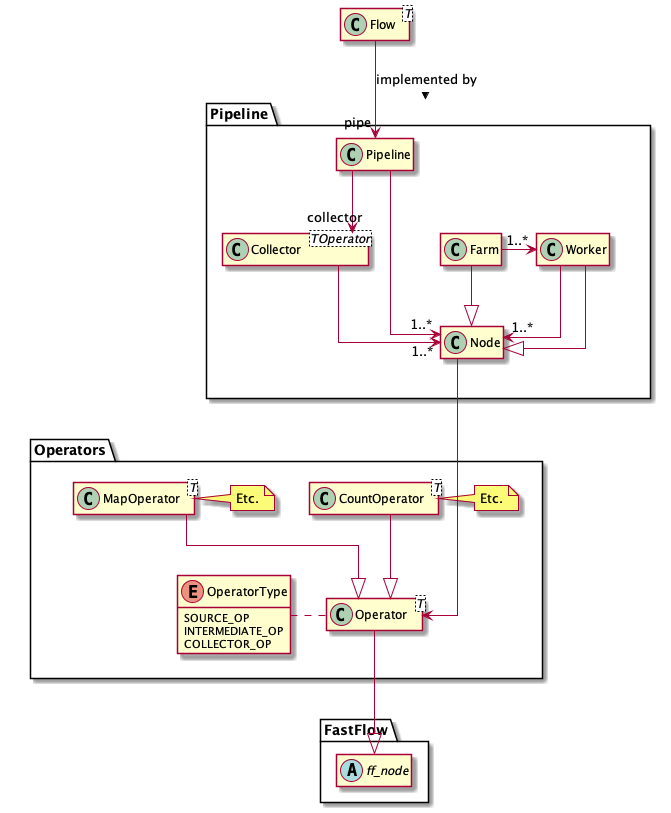
\includegraphics[width=1.0\textwidth]{Figures/vueEnsemble.png}
      \caption{Les principaux éléments (classes) de \TT{PpFf}.}
       \label{All.fig}
\end{figure}

La biblioth\`eque \TT{PpFf} est compos\'ee de plusieurs modules qui permettent de g\'erer les flux de traitement de donn\'ees. Une vue d'ensemble de ces modules est illustr\'ee dans la figure~\ref{All.fig}.

\begin{itemize}

\item Le point d'entr\'ee de \ppff\ est la classe \TT{Flow}, avec laquelle interagissent les d\'eveloppeurs pour cr\'eer des flux de traitement. Toutes les op\'erations de traitement d'un flux de \TT{PpFf} sont li\'ees aux m\'ethodes expos\'ees par cette classe. 

\item Le c\oe{}ur de la mise en \oe{}uvre de \TT{PpFf} est le module \TT{Pipeline}. La cr\'eation et l'ex\'ecution d'un flux sont g\'er\'ees par celui-ci, qui construit tout d'abord une représentation intermédaire, et qui génère ensuite un graphe de n\oe{}uds FastFlow.

\item  Le module \TT{Operators} regroupe tous les op\'erateurs d\'efinis dans \TT{PpFf}. Expos\'es \`a l'utilisateur par le biais de l'\TT{API} de \TT{PpFf}, ces op\'erateurs permettent de traiter les donn\'ees de diverses façons.

\item Le dernier module, \TT{FastFlow}, est la biblioth\`eque au–dessus de laquelle \TT{PpFf} est impl\'ement\'e.


\end{itemize}

\subsection{Flow}

\begin{figure}
\centering
     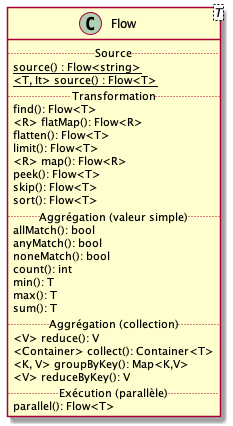
\includegraphics[width=0.5\textwidth]{Figures/flow-details.png}
      \caption{Les diff\'erentes m\'ethodes export\'ees par l'API de \TT{PpFf}.}
       \label{Flow.fig}
\end{figure}



\GT{J'ai modifié le diagramme, pour raffiner la signature générique de
certaines méthodes et \underline{aussi} pour utiliser les mêmes
groupes de méthodes que dans le chapitre précédent --- sinon c'est
mélangeant si deux terminologies/catégorisations différentes sont
utilisées.  Il faudrait donc revoir la partie ci-bas pour utiliser les
mêmes noms de groupe.}

\IC{J'ai révisé la description des groupes selon le nouveau diagramme.}


La classe \TT{Flow} est celle qui définit l'\TT{API} de la biblioth\`eque \TT{PpFf}, l'interface avec laquelle interagit le d\'eveloppeur. La figure~\ref{Flow.fig} --- qui reprend la figure~\ref{MethodesAPI.fig} --- pr\'esente la vue d'ensemble des diverses m\'ethodes export\'ees par \TT{PpFf}. Selon le type export\'e par l'\TT{API}, les m\'ethodes sont divis\'ees en plusieurs groupes : Source, Transformation, Agr\'egation et Ex\'ecution.

Source est le groupe qui permet de d\'efinir un flux de donn\'ees. En g\'en\'eral ce groupe combine les m\'ethodes qui fournissent les donn\'ees au flux. Sans un appel \`a une telle m\'ethode, un flux ne peut pas exister. Le deuxi\`eme groupe du \TT{Flow}, Transformation, est le groupe qui combine les m\'ethodes qui retournent une r\'ef\'erence vers l'objet \TT{Flow}. Ce m\'ecanisme permet d'encha\^iner les m\'ethodes de l'\TT{API}. Le troisi\`eme groupe de \TT{Flow} est le groupe Agr\'egation. Selon le type de r\'esultat produit, ce groupe est-il lui-m\^eme divis\'e en deux sous-cat\'egories : valeur simple qui combine les m\'ethodes retournant une valeur (par ex., r\'esultat bool\'een ou entier) et collection qui combine les m\'ethodes retournant une collection. Dans le dernier groupe de  \TT{Flow}, on retrouve une seule m\'ethode. Cette m\'ethode modifie le comportement d'ex\'ecution du flux. Lorsqu'elle est ajout\'ee dans le  \TT{pipeline}, toutes les op\'erations suivant cette m\'ethode seront ex\'ecut\'ees en parall\`ele en utilisant les instances d'un  \TT{farm}.

L'\TT{API} de \TT{PpFf} permet d'appliquer plusieurs op\'erations les unes à la suite des autres sur une collection de donn\'ees. Ceci est possible en encha\^inant les m\'ethodes (\emph{method chaining}). Les m\'ethodes de l'\TT{API} peuvent \^etre enchain\'ees tant qu'elles retournent une r\'ef\'erence \`a \TT{Flow}. Lorsqu'une m\'ethode retourne une valeur, une valeur simple ou une collection, le traitement est alors ex\'ecut\'e. 


\begin{lstlisting}[
label={count.c++},
language=c++,
gobble=7,
caption={Le code de la m\'ethode \TT{count} de la classe \TT{Flow} de \TT{PpFf}.},
frame=single,
float]
        unsigned int count() {
            typedef CountOperator<int> Count;
            
            pipe.addNodes<Count>(pipe.nbWorkers());
            pipe.run();

            return pipe.value<Count, int>();
        }
\end{lstlisting}

\GT{La méthode est tellement simple que tu es aussi bien de tout
donner son code! Tu peux faire un copier/coller du fichier Flow.hpp,
puis ajouter "gobble" si le code est trop indenté, pour le coller plus
à gauche.}

\IC{Je n'ai pas compris. Est-ce que je dois ajouter toutes les méthodes de Flow ?}


\GT{Puisque tu parles de mise en oeuvre, je crois que tu dois
distinguer entre le flux --- l'objet Flow --- et le pipeline qui met
en oeuvre ce flux, comme indiqué dans le diagramme donnant la vue
d'ensemble --- "implemented by".}

\IC{Merci pour cet explication. Dans ma description, j'ai vu Flow comme étant l'API et Pipeline comme le flux.}

L'\TT{API} de \TT{PpFf} est mise en œuvre par le module \TT{Pipeline}. Ce dernier s'occupe de la cr\'eation et l'ex\'ecution du flux. Le listing~\ref{count.c++} pr\'esente le code de la m\'ethode \TT{count} de l'\TT{API}. L'attribut \TT{pipe} d'un objet \TT{Flow} est une instance de la classe \TT{Pipeline}, objet qui cr\'ee et ajoute les op\'erateurs de type \TT{Count} dans le pipeline associé au flux en appelant la m\'ethode \TT{addNodes}. Une fois les n\oe{}uds ajoutés, puisqu'il s'agit d'une méthode qui produit un résultat qui n'est pas un \TT{Flow}, le traitement associé au pipeline \TT{pipe} est ex\'ecut\'e en appelant la m\'ethode \TT{run}. Puis on obtient et retourne la valeur de type entier (\TT{int}, sp\'ecifi\'e dans le deuxi\`eme param\`etre générique de la m\'ethode \TT{value}) produit par l'exécution du pipeline.

\subsection{Pipeline}
\subsection{Operateurs}


\section{Impl\'ementation de \TT{PpFf} avec \TT{FastFlow} : un exemple}


\begin{itemize}

\item objets1 

\item objets2 

\item objets3 


\end{itemize}



\chapter{Évaluation des performances~: Comparaisons de \ppff\ avec {Java} et {FastFlow}}
\label{experiences.chap}

Ce chapitre pr\'esente une \'evaluation exp\'erimentale de la biblioth\`eque \TT{PpFf} afin de comparer ses performances avec d'autres approches d'ex\'ecution parall\`ele, plus sp\'ecifiquement avec \TT{Java} et \TT{FastFlow}.
%
Dans les sections~\ref{wordcount.sect} et~\ref{stockprice.sect}, nous pr\'esentons deux applications \'ecrites avec \PpFf. Ces applications ont \'et\'e choisies non seulement pour montrer certaines fonctionnalit\'es de notre biblioth\`eque, mais \'egalement pour leur pertinence dans des sc\'enarios typiques. La section~\ref{wordcount.sect} pr\'esente une application permettant de calculer le nombre d'occurrences des mots dans un texte %
% --- le <<\emph{Hello World!}>> des syst\`emes de traitement de donn\'ees en mode \emph{batch} ---
% GT: Cette remarque, si je me souviens bien, avait été mal perçue par un des évaluateurs,
% donc il me semble préférable de l'omettre.
%
alors que la section~\ref{stockprice.sect} pr\'esente une application permettant de calculer des statistiques sur les prix d'indices boursiers --- un exemple typique de traitement de flux en ligne (\emph{online data processing}). Mais tout d'abord, nous pr\'esentons la fa\c{c}on dont nos exp\'eriences ont \'et\'e effectu\'ees.

%Finalement, la section~\ref{coutsPpFf.sect} pr\'esente une application permettant de d\'eterminer les surco\^uts introduits par \TT{PpFf} par rapport \`a \TT{FastFlow} --- un \emph{micro benchmark} consistant en un pipeline avec un seul op\'erateur. 



\section{M\'ethode utilis\'ee pour les exp\'eriences}
\label{usedMethodsForBenchmarks.chap}

\subsection{Caractéristiques des machines et compilateurs utilisés}

Chaque syst\`eme informatique a des caract\'eristiques propres. Quelques-uns des facteurs qui influencent les performances d'un tel syst\`eme sont le type de processeur, le nombre de processeurs ou de c\oe{}urs, et la vitesse des processeurs. 


\newcommand{\LARGEUR}{3cm}

\begin{table}
\begin{tabular}{|p{3cm}|p{\LARGEUR}|p{\LARGEUR}|p{\LARGEUR}|}
\hline
  & \M1 & \M2 & \M3
\\\hline
\textbf{OS} & Ubuntu 20.04.1 & CentOS 7.8.2003 & CentOS 7.6.1810
\\\hline
\textbf{Architecture} &  x86\_64 & x86\_64 & x86\_64
\\\hline
\textbf{Type de processeur} & Intel(R) Xeon(R) Gold 5120  & AuthenticAMD & Intel(R) Core(TM) i7-4790
\\\hline
\textbf{Vitesse du processeur (GHz)} & 2.20 & 2.30 & 3.96
\\\hline
\textbf{Mono/multi-usager} & Multi & Multi & Mono
\\\hline
\textbf{Nb.~coeurs physiques} & 16 & 32 & 4
\\\hline
\textbf{Nb.~coeurs logiques} & 16 & 64 & 8
\\\hline
\texttt{java}
  & \texttt{openjdk version "14.0.1" 2020-04-14}
  & \texttt{java version "1.8.0\_51"}
  & \texttt{openjdk version "11.0.7" 2020-04-14 LTS}
\\\hline
\texttt{g++ (GCC)}
   & 9.3.0
   & 8.3.1 
   & 8.3.0
\\\hline
\end{tabular}
\caption[Les caract\'eristiques des machines utilis\'ees dans les exp\'eriences.]{Les caract\'eristiques des machines utilis\'ees dans les exp\'eriences. Le tableau d\'ecrit pour chaque machine le syst\`eme d'exploitation utilis\'e, le type de la machine (mono- ou multi-usager), le nombre de coeurs (physiques vs.\ logiques) et les versions des compilateurs utilis\'es dans les exp\'eriences.}
\label{machines.table}
\end{table}


Afin d'avoir des r\'esultats plus représentatifs, nous avons conduit nos exp\'eriences sur trois machines diff\'erentes. Le tableau~\ref{machines.table} montre les caract\'eristiques de ces machines. Les machines \M1 et \M2 sont des machines multi-usagers, tandis que la machine \M3 est une machine mono-usager sur laquelle les exp\'eriences ont \'et\/e roul\'ees sans interf\'erence.
%
Soulignons que \M2 est peu utilisée et que nous étions toujours
le seul usager lorsque les expériences ont été menées. Quant aux
expériences sur \M1, le serveur \TT{labunix} le plus utilisé, elles
ont été lancées durant la nuit --- par une commande <<\TT{at 3:00AM
\ldots}>> --- alors que peu d'usagers étaient connectés

\subsection{Choix des programmes comparés}

Le fonctionnement des programmes \TT{Java}, \TT{PpFf} et~\TT{FastFlow} n'est pas le m\^eme. Alors que \TT{PpFf} et \TT{FastFlow} permettent de varier le nombre de fils d'ex\'ecution (\emph{threads}), \TT{Java} ne le permet pas. Afin de montrer les meilleurs temps d'ex\'ecution et l'\'evolutivit\'e de \TT{PpFf}, des exp\'eriences pr\'eliminaires ont \'et\'e effectu\'ees, sur chaque machine, pour identifier les meilleures versions, et ce tant pour \TT{PpFf} que pour \TT{Java} et \TT{FastFlow}.
Ces exp\'eriences pr\'eliminaires ont \'et\'e conduites avec un nombre de r\'ep\'etitions de 10 ou 20 et avec une quantit\'e <<moyenne>> ou <<grande>> de donn\'ees, selon les cas. 

Dans le cas de \TT{PpFf} et \TT{FastFlow}, l'objectif \'etait de d\'eterminer le meilleur niveau de parall\'elisme \`a utiliser dans les \emph{farm}s, c'est-\`a-dire, pour \TT{PpFf}, la valeur pour la m\'ethode \TT{parallel()}, pour le parall\'elisme de donn\'ees.
%
Par contre, dans le cas de \TT{Java}, l'objectif était de comparer diverses versions~: avec ou sans JIT, séquentielle ou parallèle, avec ou sans \emph{warmup} (voir ci-bas).
%
C'est la version parallèle avec \emph{warmup} et \emph{JIT} qui a \'et\'e utilis\'ee.%
%
\footnote{Initialement, des expériences préliminaires ont aussi été
effectuées en désactivant complètement le JIT. Toutefois, les temps
d'exécutions étaient alors tellement longs que cette variante a
rapidement été laissée de côté.}


L'effet de pr\'echauffage (\emph{warmup}) est g\'en\'eralement d\^u au chargement des classes et \`a l'interpr\'etation du \emph{bytecode} au d\'emarrage du programme plutôt qu'à l'exécution directe d'instructions machines. Lorsqu'une nouvelle application d\'emarre, toutes les classes requises sont charg\'ees en m\'emoire par le mod\`ele de chargement paresseux (\emph{lazy loading}). Un tel mod\`ele est couramment utilis\'e pour reporter l'initialisation d'un objet jusqu'au moment o\`u il est n\'ecessaire.
%
\label{jitDescription.sect}
%
Il y a aussi l'effet de la compilation 
\emph{JIT}~\citep{cramer1997compiling} (\emph{Just-In-Time compiler}),
%
un composant de l'environnement d'ex\'ecution \TT{Java} qui am\'eliore les performances des applications en compilant le \emph{bytecode} de la machine virtuelle en code machine \emph{au moment de l'ex\'ecution}. Le \emph{bytecode} est l'ensemble des instructions de la \emph{JVM} (\emph{Java Virtual Machine}) qui permet aux applications d'\^etre ex\'ecut\'ees sur plusieurs plates-formes. La conversion du \emph{bytecode} en langage machine a un impact positif significatif sur la vitesse d'ex\'ecution une fois que le code machine s'exécute directement.

Dans toutes nos exp\'eriences, les programmes \TT{Java} comparés avec \ppff\ ont donc \'et\'e pr\'echauff\'es en lan\c{c}ant une proc\'edure de pr\'echauffage avant de mesurer le temps pour la portion de code pertinente. Cette proc\'edure de pr\'echauffage a consisté à faire un traitement préalable d'une \emph{fraction} des données, traitement utilisant toutes les m\'ethodes utilis\'ees par la suite.

\subsection{Mesures des temps d'exécution}
 
Il faut noter que le temps mesur\'e dans toutes les exp\'eriences \emph{exclut le lancement du programme}. La mesure du temps se fait de l'int\'erieur du programme m\^eme, une fois celui-ci lanc\'e. Lorsque le traitement est termin\'e, le temps est \'emis en sortie du programme sur \TT{stdout}. Donc, le temps n'est pas mesur\'e avec la commande <<\TT{time}>>. Notamment, dans le cas de \TT{Java}, le temps mesuré exclut donc le temps de lancement de la machine virtuelle. De plus, les quantit\'es de donn\'ees utilis\'ees dans les exp\'eriences ont \'et\'e choisies de sorte que les temps d'ex\'ecution soient d'au moins 200 millisecondes.


\subsection{Exemples d'expériences préliminaires}

\graphe{WordCount-temps-java-11-20}{Java}

\graphe{WordCount-temps-java-2-10}{PpFf}
%\graphe{WordCount-log-temps-java-2-10}{Temps PpFf (log)}

Afin de montrer les \'etapes des diverses exp\'eriences qui ont conduit aux r\'esultats finaux, l'annexe~\ref{ExperiencesPreliminairesWordCount.ann} pr\'esente un extrait d'un fichier de configuration \TT{WordCount-bm-config.rb}, utilis\'e pour l'ex\'ecution des expériences, alors que les figures~\grapheref{WordCount-temps-java-11-20} et~\grapheref{WordCount-temps-java-2-10} présentent quelques-uns des r\'esultats préliminaires obtenus.

Cr\'e\'e par mon directeur de recherche, un script de configuration permet de décrire les expériences \`a ex\'ecuter pour une application donnée, dans notre exemple, pour \TT{WordCount}. Dans ce fichier, pour chaque expérience, on peut sp\'ecifier tous les param\`etres requis : la ou les machines sur laquelle est définie l'expérience, la quantité de donn\'ees à traiter, le nombre de r\'ep\'etitions (pour le calcul de la moyenne), et les divers programmes \`a ex\'ecuter et comparer. 

Les quantités de donn\'ees à traiter sont regroup\'ees en diverses cat\'egories, les plus importantes étant \TT{donnees\_preliminaires}, \TT{pas\_mal\_de\_donnees} et \TT{beaucoup\_de\_donnees}. Les deux premi\`eres cat\'egories ont servi pour d\'eterminer les meilleures versions \`a utiliser pour chacun des programmes (expériences préliminaires). 
%
Par exemple, les graphes des figures~\grapheref{WordCount-temps-java-11-20} et~\grapheref{WordCount-temps-java-2-10} montrent les temps d'ex\'ecution pour \TT{WordCount} sur la machine \M1 pour le programme \TT{WordCount.java} (expérience no.~11) et pour le programme \TT{WordCount.cpp}, donc version \TT{PpFf} (expériences no.~2). Les temps sont en millisecondes (ms), obtenus en prenant la moyenne de 20 ou 10 ex\'ecutions, selon le cas.
%
Pour la version \TT{Java}, quatre séries de mesures ont été
effectuées~: séquentielle sans préchauffage (\TT{Java-}), séquentielle
avec préchauffage (\TT{Java}), parallèle sans préchauffage
(\TT{Java+}), et parallèle avec préchauffage (\TT{Java*}) --- pour les résultats, voir l'annexe~\ref{wordcount-java.ann}.
%
Pour la version \ppff, trois  s\'eries de mesures ont \'et\'e effectu\'ees : \TT{PpFf-1} avec une seule instance parallèle d'un \emph{farm}, \TT{PpFf-2} avec deux et \TT{PpFf-3} avec trois.



L'objectif de ces mesures pr\'eliminaires était de d\'eterminer la valeur qui semble la meilleure pour les temps d'ex\'ecution. On peut observer que le temps d'ex\'ecution pour \TT{PpFf-3} est beaucoup plus grand que les deux autres (figure~\grapheref{WordCount-temps-java-2-10}).
%
(Pour mieux distinguer les performances entre deux ou plusieurs versions, une échelle logarithmique peut aussi être utilis\'ee, lorsque nécessaire.)
%
Pour la machine \M1, \TT{PpFf-2} est donc la version qui sera compar\'ee aux autres programmes lors des expériences finales. Ces expériences finales comparent donc les meilleures versions entre elles, en utilisant de plus grandes quantit\'es de donn\'ees et avec un plus grand nombre de r\'ep\'etitions, soit 40.


Le nombre de r\'ep\'etitions indique combien de fois chaque programme est exécuté et son temps mesuré.
%
On calcule ensuite la moyenne et l'écart-type. Dans un graphe comme celui de la figure~\grapheref{WordCount-temps-java-11-20}, les moyennes sont repr\'esent\'ees par les valeurs qui composent la courbe sur le graphe et les dispersions par des petits barres verticales (par ex., voir les valeurs pour \TT{Java+}
de la figure~\grapheref{WordCount-temps-java-11-20}). Plus précisément, la barre verticale indique un intervalle de deux (2) écart-types, donc un intervalle qui contient approximativement \emph{95~\% des temps mesurés}.%
%
\footnote{En supposant une distribution normale des temps d'ex\'ecution.}
%

Chaque s\'erie d'exp\'eriences finales inclut les versions s\'equentielles pour les programmes compar\'es des deux biblioth\`eques. Identifi\'ees sur les graphes par \TT{Seq} pour la version s\'equentielle de \TT{PpFf} et par \TT{Java} pour la version s\'equentielle avec \emph{warm-up} de \TT{Java}, ces versions utilisent les m\^emes fonctions auxiliaires que les versions parall\`eles, mais s'ex\'ecutent de fa\c{c}on strictement s\'equentielle. Ces programmes s\'equentiels ont aussi \'et\'e utilis\'e pour d\'eterminer les acc\'el\'erations. Le concept d'acc\'el\'eration d\'etermine \`a quel point un programme parall\`ele est plus rapide qu'un programme s\'equentiel \'equivalent. On distingue deux types d'acc\'elérations : relative ou absolue. Dans nos mesures, nous avons utilis\'e l'acc\'el\'eration \emph{absolue}. L'acc\'el\'eration absolue compare le programme ex\'ecut\'e sur une machine multiprocesseurs avec un programme s\'equentiel, performant, qui r\'esout le m\^eme probl\`eme. 

Afin d'illustrer aussi la dispersion des acc\'el\'erations, l'accélération moyenne a été calculée, ainsi que deux autres valeurs donnant un intervalle pour la valeur minimale et maximale de l'acc\'el\'eration. Repr\'esent\'ees aussi par des petites barres verticales dans les graphes des sections~\ref{wordcount.sect} et~\ref{stockprice.sect}, ces valeurs ainsi que l'accélération moyenne sont calcul\'ees comme suit~: 

\begin{itemize}
\item acc. moyenne  =  temps moyen séq. / temps moyen par.
\item acc. min  =  temps min séq. / temps max par.
\item acc. max = temps max séq. / temps min par.
\end{itemize}

\section{Expériences avec l'application {WordCount}}
\label{wordcount.sect}



\subsection{Description de l'application}

Dans la section~\ref{descriptionWordCount.sect}, nous avons pr\'esent\'e \TT{WordCount}, une application qui compte le nombre d'occurrences des divers mots dans un fichier texte. L'application prend en entr\'ee un fichier texte et produit un conteneur de type \TT{map<string, int>} où la cl\'e repr\'esente un mot dans le fichier et la valeur  type \TT{int}  associ\'ee repr\'esente le nombre d'occurrences du mot dans le fichier. Des extraits des programmes utilis\'es pour les exp\'eriences pour \TT{WordCount} en~\TT{Java}, \TT{C++} version \TT{Seq}uentielle, \TT{PpFf} et \TT{FastFlow} sont pr\'esent\'es dans l'annexe~\ref{appendice-code-wordcount.ann}.

\subsection{Mesures obtenues et analyse des r\'esultats}



\begin{figure}
\grapheH{WordCount-temps-java-3001-40}

\grapheH{WordCount-temps-japet-3002-40}

\grapheH{WordCount-temps-c34581-3003-40}


\caption[Les temps d'exécution des programmes pour \TT{WordCount} sur
les machines \M1, \M2 et \M3.]{Les temps d'exécution des programmes
pour \TT{WordCount} sur les machines \M1, \M2 et \M3. L'axe des $x$
indique le nombre de mots traités. L'axe des $y$ indique le temps
d'exécution, en millisecondes.}
\label{WordCount-temps.fig}
\end{figure}


\begin{figure}
\grapheH{WordCount-debits-java-3001-40}

\grapheH{WordCount-debits-japet-3002-40}

\grapheH{WordCount-debits-c34581-3003-40}


\caption[Les débits pour \TT{WordCount} sur
les machines \M1, \M2 et \M3.]{Les débits des programmes
pour \TT{WordCount} sur les machines \M1, \M2 et \M3. L'axe des $x$
indique le nombre de mots traités. L'axe des $y$ indique le nombre de
milliers de mots par seconde (K-mots/s).}
\label{WordCount-debits.fig}
\end{figure}


\begin{figure}
\grapheH{WordCount-accs-java-3001-40}

\grapheH{WordCount-accs-japet-3002-40}

\grapheH{WordCount-accs-c34581-3003-40}



\caption[Les accélérations pour \TT{WordCount} sur les machines \M1,
\M2 et \M3.]{Les accélérations des programmes pour \TT{WordCount} sur
les machines \M1, \M2 et \M3. L'axe des $x$ indique le nombre de mots
traités. L'axe des $y$ indique l'accélération absolue par rapport à
\TT{WordCountSeq.cpp} (\TT{Seq}).}
\label{WordCount-accs.fig}
\end{figure}


Dans cette section, nous \'evaluons l'application \TT{WordCount} en examinant le temps d'ex\'ecution, le d\'edit et l'acc\'el\'eration sur les trois machines : \M1, \M2 et \M3. Tel que d\'ecrit dans la section~\ref{usedMethodsForBenchmarks.chap}, des exp\'eriences pr\'eliminaires ont \'et\'e effectu\'ees afin de choisir les meilleures versions. Dans le cas de \TT{Java}, la meilleure version choisie est celle avec \emph{warmup} et \emph{JIT}. Elle est indiquée dans chaque graphe avec la notation \TT{Java*}. Dans le cas de \TT{PpFf} et \TT{FastFlow}, les exp\'eriences ont \'et\'e men\'ees en variant les nombres d'instances parall\`eles d'un \emph{farm}. Par exemple, pour \TT{PpFf}, quatre instances parall\`eles d'un \emph{farm} ont \'et\'e utilis\'es sur la machine \M1, neuf sur la machine \M2 et deux sur la machine \M3. Le suffixe entier dans les indicateurs pour \TT{PpFf} et \TT{FastFlow} dans chaque graphe repr\'esente donc ce nombre d'instances parall\`eles d'un \emph{farm}, par exemple \TT{PpFf-4} utilise quatre instances parall\`eles d'un \emph{farm}. Chaque exp\'erience inclut aussi le programme s\'equentiel, indiqué sur chaque graphe par \TT{Seq}, utilisant  les m\^emes fonctions auxiliaires que \TT{PpFf} et \TT{FastFlow}.

Les valeurs pour les unit\'es de mesures --- le temps d'ex\'ecution, le d\'ebit et l'acc\'el\'eration qui ont servi comme r\'ef\'erence pour comparer les trois programmes --- sont indiqu\'ees sur l'axe des~$y$ de chaque graphe, alors que le nombre de mots trait\'es est indiqu\'e sur l'axe des~$x$. Afin de conna\^itre l'impact de la quantit\'e de donn\'ees \`a traiter, les exp\'eriences ont \'et\'e men\'ees en utilisant plusieurs ensembles de donn\'ees. Chaque ensemble de donn\'ees --— un fichier sur disque --— contient un nombre croissant de mots. Ces nombres de mots varient de 752~856 \`a 10~185~035. Les r\'esultats finaux sont des moyennes pour 40~r\'ep\'etitions. Ils sont pr\'esent\'es comme suit : 



\begin{itemize}

\item Figure~\ref{WordCount-temps.fig}~: les temps
d'ex\'ecution sur les machines \M1, \M2 et \M3.

\item Figure~\ref{WordCount-debits.fig}~: les débits sur \M1, \M2 et \M3.

\item Figure~\ref{WordCount-accs.fig}~: les accélérations
par rapport à la version \TT{Seq}entielle
sur \M1, \M2 et \M3.
\end{itemize}


Il faut pr\'eciser que pour \TT{WordCount}, le r\'esultat n'est pas tri\'e. Du point de vue de la parall\'elisation, le tri est plut\^ot lie \'a l'algorithme de tri et non \`a la parall\'elisation. Pour toutes les versions, c'est un \emph{dictionnaire} qui est produit --- \TT{unordered\_map} en \TT{C++}, \TT{HashMap} en \TT{Java} --- et la mesure du temps d'exécution se termine une fois le \emph{dictionnaire} construit.


En comparant les temps d'ex\'ecution entre \TT{PpFf} et \TT{Java}, on constate que, pour les machines \M1 et \M3, \TT{Java} est plus performant que \TT{PpFf}. La gestion de \emph{threads} entre les deux programmes diff\`ere. \TT{PpFf} ex\'ecute chaque op\'eration d'un \TT{pipeline} sur un \emph{thread} diff\'erent. Par exemple, les cinq op\'erations de \TT{WordCount} --- \TT{source}, \TT{flatMap}, \TT{map}, \TT{find} et \TT{reduceByKey} --- s'ex\'ecutent sur cinq \emph{threads} diff\'erents. Par contre, \TT{Java} g\`ere la cr\'eation de \emph{threads} par l'interm\'ediaire du \emph{framework} \TT{fork/join}. D\'ecrit dans le chapitre~\ref{outils_connus.chap}, le \emph{framework} divise une t\^ache en plus petites sous-t\^aches ind\'ependantes, et ce r\'ecursivement jusqu'\`a ce qu'elles soient assez simples pour \^etre ex\'ecut\'ees, et ce de façon efficace grâce à une approche de \emph{work stealing}~\citep{FrigoLeiRan98}. Ce m\'ecanisme permet \`a \TT{Java} d'\^etre plus efficace que \TT{PpFf} sur les machines \M1 et \M3. \TT{PpFf} est plus rapide que \TT{Java} sur la machine \M2. La figure~\ref{WordCount-debits.fig}, machine \M2, montre cet aspect. Par rapport aux machines \M1 et \M3, \M2 dispose d'un plus grand nombre de processeurs. Cela a permis d'augmenter le nombre d'instances parall\`eles d'un \emph{farm} dans le programme \TT{PpFf} et en cons\'equence \TT{PpFf} est plus performant que \TT{Java}. 


En comparant les temps d'ex\'ecution entre les programmes \TT{PpFf} et \TT{FastFlow}, on constate que \TT{PpFf} obtient presque le m\^eme temps d'ex\'ecution que \TT{FastFlow} sur la machine \M3 et qu'il performe mieux que \TT{FastFlow} sur les machines \M1 et \M2. On rappelle que \TT{PpFf} est impl\'ement\'e au–dessus de la biblioth\`eque \TT{FastFlow}, et donc il semble que \TT{PpFf} n'introduise pas de surco\^uts par rapport \`a \TT{FastFlow}. 

Afin de mieux comparer les deux programmes, \TT{PpFf} et \TT{Java}, nous avons aussi calculé, à partir des mêmes séries d'exp\'eriences, le d\'ebit, soit le nombre de mots trait\'e par seconde. Tel qu'on peut le voir dans la figure~\ref{WordCount-debits.fig}, ces débits ont \'et\'e calculés pour les trois machines. L'axe des $x$ indique le nombre de mots trait\'es et l'axe des $y$ indique le nombre de milliers de mots par seconde (\TT{K-mots/s}). Un point int\'eressant, qui peut \^etre observ\'e dans les diagrammes de d\'ebits, est que le d\'ebit est relativement constant. En prenant comme exemple le diagramme pour \TT{PpFf-4} pour \M1 de la figure~\ref{WordCount-debits.fig}, on peut noter que le d\'ebit reste relativement stable peu importe la taille du fichier. Cela d\'emontre que \TT{PpFf} est efficace non seulement pour un petit volume de travail, mais aussi pour de grands traitements de donn\'ees.

La derni\`ere s\'erie de résultats tirée de nos exp\'eriences vise \`a comparer les acc\'el\'erations. Illustr\'ees sur la figure~\ref{WordCount-accs.fig}, les acc\'el\'erations indiquent \`a quel point un programme parall\`ele est plus rapide qu'un programme s\'equentiel \'equivalent. En comparant les acc\'el\'erations du programme \TT{PpFf} avec celles de \TT{FastFlow}, on peut observer que \TT{PpFf} a de meilleures acc\'elérations sur les machines \M1 et \M2 et une acc\'elération presque identique sur la machine \M3. Cela montre que \TT{PpFf} n'introduit pas des surco\^uts par rapport \`a \TT{FastFlow}. Par contre, \TT{Java} a de meilleures acc\'el\'erations pour \M1 et \M3, mais pas pour \M2. Comme on peut le constater dans le tableau~\ref{machines.table}, la machine \M2 dispose d'un plus grand nombre de processeurs par rapport \`a \M1 et \M3. Cet avantage est exploit\'e par les instances de \emph{farm}, permettant \`a \TT{PpFf} d'obtenir une meilleure acc\'el\'eration que \TT{Java} sur cette machine.



\section{Expériences avec l'application {StockPrice}}
\label{stockprice.sect}

Dans le monde informatique actuel, les institutions financi\`eres produisent d'\'enormes quantit\'es d'informations, par ex., des informations sur les march\'es boursiers. Un probl\`eme important qu'elles rencontrent consiste \`a trouver des moyens efficaces pour r\'esumer et visualiser les donn\'ees afin de produire des informations utiles sur le comportement du march\'e, notamment pour prendre des d\'ecisions d'investissement. Cette section pr\'esente une application qui calcule le prix maximum pour diverses actions d'un marché boursier. Des extraits des programmes utilis\'es pour les exp\'eriences pour \TT{StockPrice} en~\TT{Java}, \TT{C++} version \TT{Seq}uentielle, \TT{PpFf} et \TT{FastFlow} sont pr\'esent\'es dans l'annexe~\ref{appendice-code-stockprice.ann}.


\subsection{Description de l'application}

L'application \TT{StockPrice} calcule le prix d'une action en utilisant le modèle \emph{Black-Scholes}~\citep{macbeth1979empirical}. Ce mod\`ele d'\'evaluation est utilis\'e pour d\'eterminer le prix juste ou la valeur th\'eorique d'une option d'achat ou de vente, et ce en fonction de six variables telles que la valeur de l'action sous-jacente, le prix d'exercice, le taux d'int\'er\^et sans risque, la volatilit\'e du prix de l'action, la dur\'ee et le type d'option. 
%
Les calculs associés à cette évaluation sont assez simples en termes
algorithmiques, puisqu'il s'agit essentiellement d'une séquence
linéaire de calculs points-flottants.

\begin{lstlisting}[float,label={StockPrice-code.listing},gobble=4,basicstyle=\ttfamily\footnotesize,language=c++,caption={Un extrait du code de \TT{StockPrice.cpp} (version \ppff).},frame=single]
    Reducer<StockAndPrice, double>
       reducer(0.0, 
               [](double maxPrice, StockAndPrice sp) {
                  return std::max(maxPrice, sp.StockPrice);
               },
               [](double max, double workerResult) { 
                  return std::max(max, workerResult);
               });
    std::unordered_map<std::string, double> currentResult =
        Flow
        ::source(inputFile)
        .parallel(nbFarmWorkers)
        .map<std::string, OptionData>(getOptionData)
        .map<OptionData, StockAndPrice>(calculateStockPrice)
        .reduceByKey<StockAndPrice, std::string, double>(
               reducer, 
               [](StockAndPrice* sp) { return &(sp->StockName); } );
\end{lstlisting}


L'application \TT{StockPrice} est compos\'ee de cinq op\'erations principales, comme on peut le voir dans le listing~\ref{StockPrice-code.listing} qui présente un extrait de la version \ppff.

\begin{lstlisting}[
label={exampleInfoActionFromFile},
language=c++,
caption={Un exemple illustrant l'information sur des actions contenues dans le fichier.},
frame=single,
float]
SNY 100.00 90.00 0.1000 0.00 0.10 1.00 C 0.00 18.6308591206674982
JCI 100.00 100.00 0.1000 0.00 0.10 0.50 C 0.00 5.8502736042849798
DSX 100.00 100.00 0.1000 0.00 0.10 1.00 C 0.00 10.3081472436668
LILA 100.00 110.00 0.1000 0.00 0.10 0.10 C 0.00 0.003523074865
NVS 100.00 110.00 0.1000 0.00 0.10 0.50 C 0.00 1.1407228438274099
FLML 100.00 110.00 0.1000 0.00 0.10 1.00 C 0.00 4.216747020308
TEF 100.00 90.00 0.1000 0.00 0.25 0.10 C 0.00 11.1352446183467002
DXB 100.00 90.00 0.1000 0.00 0.25 0.50 C 0.00 16.0926388440922991
HSEA 100.00 90.00 0.1000 0.00 0.25 1.00 C 0.00 21.16345465848
LENS 100.00 100.00 0.1000 0.00 0.25 0.10 C 0.00 3.65996266031
\end{lstlisting}


\begin{itemize}

\item Une op\'eration \TT{Flow::source} qui d\'efinit la source du flux de donn\'ees. Ici, la source est constitu\'ee par les lignes contenues dans un fichier. Le listing~\ref{exampleInfoActionFromFile} montre un exemple avec quelques enregistrements tir\'es d'un des fichiers de données. 


\medskip

Un enregistrement est identifi\'e par les informations suivantes : le nom de l'action, la valeur actuelle de l'action sous-jacente, le prix d'exercice, le taux d'int\'er\^et sans risque, le taux de dividende, la volatilit\'e du prix de l'action, le temps qu'il reste \`a l'option avant son \'ech\'eance (exprim\'e en ann\'ees), le type d'option (\TT{C=CALL}~: prix pour une option d'achat~; \TT{P=PUT}~: prix pour une option de vente), la valeur de dividende et la valeur de r\'ef\'erence \TT{DerivaGem}. 
Les valeurs \TT{DerivaGem}, la valeur et le taux de dividende ne sont pas utilis\'es dans \TT{StockPrice} pour calculer le prix d'une action.

\item Une op\'eration \TT{parallel} qui r\'epartit les \'el\'ements du flux entre divers \emph{threads} de parallélisme de données.
Toutes les \'etapes qui suivent cette op\'eration seront donc ex\'ecut\'ees en parall\`ele, via une \emph{farm}.

\item Une op\'eration \TT{map}, qui permet d'extraire le nom et les options de chaque action.

\item  Une autre op\'eration \TT{map} qui calcule le prix de chaque action. L'algorithme utilis\'e est celui de \emph{Black-Scholes}~\citep{macbeth1979empirical}. 

\item Une derni\`ere op\'eration, \TT{reduceByKey}, qui extrait le prix maximum pour chaque action.

\end{itemize}

\subsection{Mesures obtenues et analyse des r\'esultats}


\begin{figure}
\grapheH{StockPrice-temps-java-3001-40}

\grapheH{StockPrice-temps-japet-3002-40}

\grapheH{StockPrice-temps-c34581-3003-40}


\caption[Les temps d'exécution des programmes pour \TT{StockPrice} sur
les machines \M1, \M2 et \M3.]{Les temps d'exécution des programmes
pour \TT{StockPrice} sur les machines \M1, \M2 et \M3. L'axe des $x$
indique le nombre de transactions traitées. L'axe des $y$ indique le temps d'exécution, en millisecondes.}
\label{StockPrice-temps.fig}
\end{figure}


\begin{figure}
\grapheH{StockPrice-debits-java-3001-40}

\grapheH{StockPrice-debits-japet-3002-40}

\grapheH{StockPrice-debits-c34581-3003-40}


\caption[Les débits pour \TT{StockPrice} sur
les machines \M1, \M2 et \M3.]{Les débits des programmes
pour \TT{StockPrice} sur les machines \M1, \M2 et \M3. L'axe des $x$
indique le nombre de transactions traitées. L'axe des $y$ indique le nombre de milliers de transactions par seconde (K-transactions/s).}
\label{StockPrice-debits.fig}
\end{figure}


\begin{figure}
\grapheH{StockPrice-accs-java-3001-40}

\grapheH{StockPrice-accs-japet-3002-40}

\grapheH{StockPrice-accs-c34581-3003-40}


\caption[Les accélérations pour \TT{StockPrice} sur les machines \M1,
\M2 et \M3.]{Les accélérations des programmes pour \TT{StockPrice} sur
les machines \M1, \M2 et \M3. L'axe des $x$ indique le nombre de mots
traités. L'axe des $y$ indique l'accélération absolue par rapport à
\TT{StockPriceSeq.cpp} (\TT{Seq}).}
\label{StockPrice-accs.fig}
\end{figure}


Dans cette section, nous \'evaluons l'application \TT{StockPrice} en examinant le temps d'ex\'ecution, le d\'ebit et l'accélération sur les trois machines : \M1, \M2 et \M3. 

Comme dans le cas de \TT{WordCount}, des exp\'eriences pr\'eliminaires ont \'et\'e effectu\'ees afin de choisir les meilleures versions. Dans le cas de \TT{Java}, la meilleure version choisie est celle avec \emph{warmup} et \emph{JIT}. Elle est indiqu\'ee dans chaque graphe avec la notation \TT{Java*}. Dans le cas de \TT{PpFf} et \TT{FastFlow}, les exp\'eriences ont \'et\'e men\'ees en variant les nombres d'instances parall\`eles d'un \emph{farm}. Les meilleures versions choisies pour \TT{PpFf} (resp.\ \TT{FastFlow}) sont celles utilisant cinq et quatre (resp.\ quatre et quatre) instances parall\`eles d'un \emph{farm} sur les machines \M1 et \M2 et deux sur la machine \M3. Comme pour \TT{WordCount}, le suffixe entier dans les indicateurs pour \TT{PpFf} et \TT{FastFlow} dans chaque graphe repr\'esente donc ce nombre d'instances parall\`eles d'un \emph{farm}. Chaque exp\'erience inclut aussi le programme s\'equentiel, indiqu\'e sur chaque graphe par \TT{Seq}. Chaque programme calcule le prix maximum pour plusieurs actions. Les temps d'ex\'ecution et les d\'ebit r\'esultants sont repr\'esent\'es sur l'axe des~$y$ de chaque graphe, alors que les nombres de transactions trait\'ees sont repr\'esent\'es sur l'axe des~$x$. Les r\'esultats de exp\'eriences finaux sont des moyennes pour 40 r\'ep\'etitions. Ils sont pr\'esent\'es comme suit :


\begin{itemize}

\item Figure~\ref{StockPrice-temps.fig}~: les temps d'ex\'ecution sur les machines \M1, \M2 et \M3.

\item Figure~\ref{StockPrice-debits.fig}~: les d\'ebits sur les machines \M1, \M2 et \M3.

\item Figure~\ref{StockPrice-accs.fig}~: les accélérations sur les machines \M1, \M2 et \M3.

\end{itemize}


En examinant les temps d'ex\'ecution sur les trois machines, on peut constater que \TT{Java} est plus rapide que \TT{PpFf}. On verra dans la section~\ref{limitesppff.sect} pourquoi \TT{Java} est plus performant. Par contre, si on compare \TT{PpFf} et \TT{FastFlow}, les diff\'erences des temps d'ex\'ecution sont faibles. Cela d\'emontre que les surco\^uts introduits par \TT{PpFf} par rapport \`a \TT{FastFlow} sont négligeables.

\`A partir des m\^emes s\'eries d'exp\'eriences, nous avons aussi calcul\'e les d\'ebits, soit le nombre de transactions trait\'ees par seconde. Dans la figure~\ref{StockPrice-debits.fig}, on trouve les d\'ebits moyens, indiqués par les valeurs qui composent la courbe sur le graphe, ainsi que des petites barres verticales qui indiquent la dispersion de débits mesurés~; comme pour \TT{WordCount}, cet intervalle indique la moyenne $\pm$ deux fois l'écart-type. Un point int\'eressant, qui peut \^etre observ\'e dans les graphes de d\'ebits, est que la dispersion du d\'ebit pour \TT{Java} est plus grande que celle de \TT{PpFf}. 
%
Nous avons aussi calculé les accélérations, présentées dans la
figure~\ref{StockPrice-accs.fig}~: on constate que les accélérations sur \M2 et \M3 ne sont pas très bonnes.

\section{Autres expériences avec l'application {WordCount}~: Utilisation de \TT{parallel} et nombre de \emph{threads}} 
\label{autres-experiences-wordcount.sect}

On a vu dans la plupart des exp\'eriences présentées dans les sections précédentes que notre biblioth\`eque \TT{PpFf} est généralement moins performante que \TT{Java}. Cela est d\^u \`a la gestion de \emph{threads} qui diff\`ere entre les deux programmes. Dans cette section, nous analysons plus en détail le fonctionnement et la gestion de \emph{threads} de \TT{PpFf}. 

La cr\'eation d'un \emph{thread} est une opération co\^uteuse. La surcharge varie selon les plates-formes, mais la cr\'eation d'un \emph{thread} requiert toujours l'exécution d'un grand nombre d'instructions additionnelles. Si le traitement effectué par un \emph{thread} est trop petit, il devient inutile d'avoir ce \emph{thread} puisque les surcoûts peuvent être aussi grands que le traitement lui-même. Donc, afin d'amortir les co\^uts li\'es \`a la cr\'eation d'un \emph{thread}, il faut avoir suffisamment de travail à faire faire par le \emph{thread} pour que cela en vaille la peine.

Les exp\'eriences présentées dans cette section vont d\'emontrer que la charge de travail associée à un opérateur influence fortement le temps d'ex\'ecution, et que s'il est trop petit, les performances parallèles diminuent.


\subsection{Description de trois variantes de {WordCount}}

L'application choisie pour ces exp\'eriences est l'application \TT{WordCount}, d\'ecrite dans la section~\ref{descriptionWordCount.sect}. Afin de montrer les coûts associés à la gestion des \emph{threads}, trois versions de \TT{WordCount} vont être comparées : \TT{WordCountSplitted} avec un pipeline comptant cinq op\'erations, \TT{WordCount} avec quatre opérations, et \TT{WordCountMerged} avec seulement trois op\'erations. On doit pr\'eciser que le r\'esultat obtenu en ex\'ecutant les trois versions de \TT{WordCount} est identique et que l'appel à \TT{parallel()} (voir ci-bas) n'est pas compté dans les opérations. Des extraits du code utilis\'e pour la définition de trois versions sont pr\'esent\'es dans l'annexe~\ref{appendice-code-wordcount-sf.ann}. 

\goodbreak
Les cinq op\'erations du pipeline pour \TT{WordCountSplitted} sont les suivantes :
\begin{enumerate}
\item \TT{source}, pour extraire et retourner un flux avec les lignes du fichier sp\'ecifi\'e en argument.

Note~: Dans tous les cas, l'appel à \TT{source} est immédiatement suivi d'un appel à \TT{parallel}, la m\'ethode qui permet de r\'epartir les \'el\'ements du flux entre divers sous-flux et \emph{threads}.

\item \TT{map}, pour d\'ecomposer chaque ligne en une collection de mots.

\item \TT{flatten}, pour d\'ecomposer une collection de mots en mots individuels.

\item \TT{map}, pour transformer chacun des mots en rempla\c{c}ant les lettres majuscules en minuscules.

\item \TT{reduceByKey}, pour regrouper les mots similaires ensemble et compter le nombre d'occurrences de chaque mot.
\end{enumerate}

La version \TT{WordCount} est cr\'e\'ee \`a partir de la version \TT{WordCountSplitted} en \emph{fusionnant} les appels aux m\'ethodes \TT{map} et \TT{flatten}, qui sont remplac\'es par un appel à \TT{flatMap}.

Finalement, 
la version \TT{WordCountMerged} est cr\'e\'ee \`a partir de \TT{WordCount} en fusionnant les appels aux m\'ethodes \TT{flatMap} et \TT{map}. Plus précisément, ces deux étapes sont fusionn\'ees en combinant en une seule fonction l'argument fourni à \TT{flatMap} et celui fourni à \TT{map}. Donc, comme on peut le noter dans l'annexe~\ref{appendice-code-wordcount-f.ann}, les fonctions \TT{splitInWords} et \TT{toLowercaseLetters} (pass\'ees en argument à \TT{flatMap} et \TT{map}) sont remplac\'ees par la fonction \TT{splitInLowerCaseWords} (passée en argument au \TT{flatMap} de \TT{WordCountMerged}).

\newcommand{\TO}{$\rightarrow$}

Donc, en résumé~:

{\small
\begin{centering}
\begin{tabular}{lllllll}
\TT{WordCountSplitted} & = & \TT{source} \TO & \TT{map} \TO & \TT{flatten} \TO & \TT{map} \TO & \TT{reduceByKey}
\\
\TT{WordCount} & = & \TT{source} \TO & \TT{flatMap} & \TO & \TT{map} \TO & \TT{reduceByKey}
\\
\TT{WordCountMerged} & = & \TT{source} \TO & \TT{flatMap'} & \TO & & \TT{reduceByKey}
\end{tabular}
\end{centering}
}

\subsection{Mesures obtenues et analyse des r\'esultats}


\begin{figure}
\grapheH{WordCount-temps-c34581-2003-40}

\grapheH{WordCount-temps-c34581-20031-40}

\caption[Les temps d'exécution des programmes pour \TT{WordCount}
sur la machine \M3.]{Les temps d'exécution des
programmes pour \TT{WordCount} sur la machine \M3. L'axe des $x$ indique le nombre de mots traités. L'axe des $y$
indique le temps d'exécution, en millisecondes.}
\label{WordCount-merged-splitted-temps.fig}
\end{figure}

Nous allons maintenant \'evaluer les trois versions de \TT{WordCount} en examinant les temps d'ex\'ecution sur la machine \M3. Deux s\'eries d'exp\'eriences ont \'et\'e men\'ees en variant les nombres d'instances parall\`eles d'un \emph{farm}. Dans la premi\`ere s\'erie, nous avons utilis\'e deux instances parall\`eles d'un \emph{farm} et dans la deuxi\`eme seulement une instance.  Les r\'esultats sont présentés dans la figure~\ref{WordCount-merged-splitted-temps.fig}. Les trois versions \TT{WordCountSplitted}, \TT{WordCount} et \TT{WordCountMerged} sont identifiées sur les graphes par \ppffs, \ppff\ et \ppffm\ suivi d'un suffixe entier, qui repr\'esente le nombre d'instances parall\`eles d'un \emph{farm}. Par exemple, \ppffs\TT{-2} repr\'esente la version du programme \TT{WordCountSplitted} qui utilise deux instances parall\`eles d'un \emph{farm} (\TT{parallel(2)}).

On rappelle que, dans \TT{PpFf}, chaque op\'eration ajout\'ee dans le pipeline de traitement d'un flux s'ex\'ecute sur un \emph{thread} diff\'erent (parallélisme de flux). Le traitement peut \^etre davantage parall\'elis\'e si on utilise aussi les instances parall\`eles d'un \emph{farm} (parallélisme de données), instances qui sont cr\'e\'ees en encha\^inant la m\'ethode \TT{parallel}. La valeur enti\`ere pass\'ee en argument de cette m\'ethode sp\'ecifie le nombre d'instances parall\`eles d'un \emph{farm} entre lesquelles sont r\'epartis les \'el\'ements du flux \`a traiter. Par exemple, si la valeur de l'argument est 1, les versions \TT{WordCountSplitted}, \TT{WordCount} et \TT{WordCountMerged} sont ex\'ecut\'ees en utilisant repsectivement cinq, quatre et trois \emph{threads}, correspondant aux op\'erations (étages) de leur pipeline de traitement. Par contre, si la valeur pass\'ee en argument \`a  \TT{parallel} est~2, le flux est divis\'e en deux sous-flux et chaque op\'eration du pipeline après la m\'ethode \TT{parallel} est ex\'ecut\'ee sur un \emph{thread} diff\'erent pour chaque sous-flux. Par exemple, \TT{WordCountSplitted} avec \TT{parallel(2)} est ex\'ecut\'ee en utilisant~9~\emph{threads}, un \emph{thread} correspondant \`a la m\'ethode \TT{source} et les autres 8 \emph{threads} correspondant aux~4~op\'erations qui suivent, qui sont toutes ex\'ecut\'ees sur deux instances parall\`eles d'un \emph{farm}.

En comparant les temps d'ex\'ecution pour les trois versions de \TT{WordCount} pour la premi\`ere s\'erie d'exp\'eriences, avec \TT{parallel(2)}, on constate que \TT{WordCountMerged} est plus performant que les deux autres. Pour le m\^eme travail \`a ex\'ecuter, \TT{WordCountMerged} utilise seulement trois op\'erations par rapport aux versions \TT{WordCount} et \TT{WordCountSplitted} qui utilisent quatre et cinq opérations. Comme chaque op\'eration est ex\'ecut\'ee sur un \emph{thread} diff\'erent \emph{pour chaque sous-flux cr\'e\'e}, \TT{WordCountMerged} utilise moins de \emph{threads} pour la m\^eme tache \`a accomplir, et donc les co\^uts introduits par la cr\'eation des \emph{threads} sont moins importants. Cela peut \^etre observ\'e sur le graphe o\`u, pour une valeur maximale de mots \`a traiter, \TT{WordCountMerged} obtient un meilleur temps d'ex\'ecution que \TT{WordCount} de 0.5s et de plus de 1s que \TT{WordCountSplitted}. 

Dans la deuxi\`eme s\'erie d'exp\'eriences, avec l'utilisation de \TT{parallel(1)}, les diff\'erences de temps d'ex\'ecution entre les trois versions de programmes sont beaucoup plus petites. L'utilisation d'une seule instance parall\`ele d'un \emph{farm} entra\^ine l'utilisation d'un seul \emph{thread} suppl\'ementaire entre les versions de programmes. Par exemple, la version \TT{WordCount} ex\'ecut\'ee en utilisant quatre \emph{threads} est légèrement plus rapide (4419.6 ms) que la version \TT{WordCountSplitted} qui utilise cinq \emph{threads} (4526.6 ms). 

Malgr\'e les coûts qui lui sont associés, le parall\'elisme de données dans \TT{PpFf} reste important. Cela peut \^etre constat\'e si on compare les temps moyens d'ex\'ecution pour la m\^eme s\'erie d'exp\'eriences, \TT{parallel(1)}, entre la version \TT{WordCountMerged} et les deux autres versions. En utilisant trois \emph{threads}, la version \TT{WordCountMerged} avec un temps d'ex\'ecution de 4569.6 ms est moins performante que les versions \TT{WordCount} (4 \emph{threads}) et \TT{WordCountSplitted} (5~\emph{threads}). Cet effet est plus \'evident si on compare les temps d'ex\'ecution entre les deux s\'eries d'exp\'eriences. Les versions avec \TT{parallel(2)} --- \ppffs\TT{-2} (3730.5 ms), \ppff\TT{-2} (3079.8 ms) et \ppffm\TT{-2} (2479.9 ms) --- sont plus rapides que les versions avec \TT{parallel(1)} --- \ppffs\TT{-1} (4526.6 ms), \ppff\TT{-1} (4419.6 ms) et \ppffm\TT{-1} (4569.6 ms).




\section{Discussion des résultats et limites de PpFf}
\label{limitesppff.sect}

Dans ce chapitre, plusieurs exp\'eriences ont \'et\'e présentées dans le but d'évaluer les performances de \TT{PpFf}.

Tout d'abord, deux applications utilisant \TT{PpFf} ont \'et\'e compar\'ees avec des programmes \TT{Java} \'equivalents utilisant les \TT{Streams}. Diverses unit\'es de mesures --– temps d'ex\'ecution, d\'ebit et acc\'elération --- ont servi comme r\'ef\'erence pour comparer ces programmes. Les r\'esultats de ces exp\'eriences ont montr\'e que \TT{Java} se comporte généralement mieux, ais pas toujours, que \TT{PpFf}. 
%
Ces mêmes exp\'eriences ont aussi permis de comparer \TT{PpFf} avec \TT{FastFlow}. Les r\'esultats ont montr\'e que les surco\^uts introduits par \TT{PpFf} sont peu \'elev\'es.


Ensuite, d'autres exp\'eriences ont \'et\'e men\'ees pour comparer diff\'erentes versions du programme \TT{WordCount}, versions cr\'e\'ees enti\`erement \`a l'aide de la biblioth\`eque \TT{PpFf}.
%
% Ces exp\'eriences ont montr\'e que \TT{PpFf} reste une biblioth\`eque assez efficace.
%
Ces expériences nous ont montré que lorsqu'un trop grand nombre de
\emph{threads} sont créés, le programme devient moins efficace.

Un programme cr\'e\'e en utilisant la biblioth\`eque \TT{PpFf} peut \^etre d\'ecompos\'e en diff\'erents \'etages (\'etapes), \'etages qui repr\'esentent les op\'erations à effectuer dans la cha\^ine de traitement d'un flux. Con\c{c}u dans un style fonctionnel, \TT{PpFf} permet de d\'ecomposer un programme en fines t\^aches. Or, la taille d'une telle t\^ache --- sa granularit\'e --- qui repr\'esente le travail dans un \'etage, influence fortement les temps d'ex\'ecution du programme. Les r\'esultats des exp\'eriences de la section~\ref{autres-experiences-wordcount.sect} ont montr\'e que si la granularit\'e est trop fine et qu'il y a trop de \emph{threads}, le programme résultant sera moins performant. 

Donc, la d\'ecomposition en \'etages est importante et utile, mais il faut s'assurer que le travail fait par un \'etage soit assez gros, sinon les surco\^uts du parall\'elisme deviennent trop grands.
%
Nous reviendrons sur cette question dans la conclusion, dans la partie sur les travaux futurs.




%%%%%%%%%%%%%%%%%%%%%%%%%%%%%%%%%%%%%%%%%%%%%
%%%%%%%%%%%%%%% Conclusion %%%%%%%%%%%%%%%%%%
%%%%%%%%%%%%%%%%%%%%%%%%%%%%%%%%%%%%%%%%%%%%%


\begin{conclusion}
\label{conclusion.chap}

Dans ce m\'emoire, nous avons pr\'esent\'e \TT{PpFf}, une API qui peut \^etre utilis\'ee pour cr\'eer des applications de traitement de flux de donn\'ees. Impl\'ement\'ee par l'interm\'ediaire de la biblioth\`eque \TT{FastFlow} et \TT{C++ 17}, l'\TT{API} exploite les fonctionnalit\'es modernes du \TT{C++} et les concepts de programmation g\'en\'erique.

Con\c{c}ue au-dessus de la biblioth\`eque \TT{FastFlow}, \TT{PpFf} fournit une abstraction de programmation souple et expressive qui facilite le d\'eveloppement d'applications parall\`eles, masquant ainsi non seulement la complexit\'e des m\'ecanismes de traitement concurrent, mais aussi le mod\`ele et le traitement de donn\'ees utilis\'es. L'abstraction dans \TT{PpFf} vise \`a simplifier la mani\`ere dont une s\'equence de donn\'ees est visualis\'ee et trait\'ee, permettant ainsi de r\'eutiliser les m\^emes op\'erateurs dans diff\'erents contextes et de r\'eutiliser les m\^emes algorithmes sur diff\'erents mod\`eles de donn\'ees (par exemple \TT{vector}, \TT{list}, \TT{set} etc.). Ces aspects diff\'erencient notre \TT{API} d'autres \TT{API} qui exposent diff\'erents types de donn\'ees \`a utiliser dans la m\^eme interface, ce qui oblige le d\'eveloppeur \`a r\'e\'evaluer ses op\'erations lorsque le contexte change.

Avec une \TT{API} claire et simple, \TT{PpFf} a \'et\'e con\c{c}u dans un style fonctionnel. Il expose donc \`a l'utilisateur un ensemble de m\'ethodes qui peuvent \^etre cha\^in\'ees afin de transformer les donn\'ees dans un style purement fonctionnel \`a l'aide d'une s\'erie de transformations.


Les r\'esultats d'exp\'eriences montrent que \TT{PpFf} peut fournir des applications de traitement de flux de donn\'ees \`a haut d\'ebit. Les bonnes performances obtenues par \TT{PpFf} sont d\^ues en partie au fait qu'il b\'en\'eficie directement de la conception optimis\'ee de \TT{FastFlow} pour le traitement de flux.

En ex\'ecutants diff\'erents tests, \TT{PpFf} a d\'emontr\'e la facilit\'e avec laquelle son \TT{API} permet de r\'esoudre certains probl\`emes classiques de traitement de flux de donn\'ees. Sa conception permet d'utiliser de nombreux concepts de programmation fonctionnels, par exemple, les \TT{lambdas} ou l'\'evaluation paresseuse. Ces aspects font de \TT{PpFf} un outil puissant.

Dans le chapitre sur les exp\'eriences nous avons \'egalement montr\'e que, dans certains cas, notre \TT{API} pouvait obtenir de meilleurs temps d'ex\'ecution qu'un programme \TT{Java} \'equivalent, avec les \TT{Stream}s introduits en Java 8.0, l'un des outils de traitement de donn\'ees le plus performant de nos jours.

Avec \TT{PpFf}, nous croyons que \TT{C++} a une chance de rivaliser avec \TT{Java} qui est consid\'er\'e souvent comme plus convivial que \TT{C++}. 


\section*{\textbf{Perspectives}}

Les travaux pr\'esent\'es dans ce m\'emoire pourraient \^etre \'etendus dans plusieurs directions, dont certaines sont d\'ecrites ci-dessous.

\textbf{Ajouter de nouvelles m\'ethodes parall\`eles} Afin de construire des requ\^etes compl\`etes sur une s\'equence de donn\'ees, nous pourrions \'etendre \TT{PpFf} pour prendre en charge davantage de m\'ethodes parall\`eles de traitement de flux et de donn\'ees, par exemple, \TT{distinct}, \TT{findAny}, \TT{findFirst}, \TT{forEach}, \TT{of}, etc. Ceci donnerait \`a l'utilisateur une plus grande flexibilit\'e pour la manipulation de donn\'ees.

\textbf{Optimiser la génération du graphe FastFlow} L'une des caract\'eristiques de \TT{PpFf} est que chaque op\'eration dans la cha\^ine de traitement s'ex\'ecute sur un \emph{thread} diff\'erent. Comme on l'a vu dans le chapitre sur les expérimentations, cela peut affecter les performances d'un programme si le travail fait par une op\'eration n'est pas assez important pour compenser les surco\^uts introduits par la cr\'eation de \emph{threads}. Afin d'optimiser le graphe généré, il serait intéressant d'impl\'ementer un module qui fusionne des op\'erations lorsque le travail fait par une op\'eration semble trop court, trop simple. Pour ce faire, il faudrait aussi définir un modèle de coûts, pour estimer cette quantité de travail.

\textbf{Impl\'ementer un syst\`eme distribu\'e} La version actuelle de \TT{PpFf} est con\c{c}ue pour fonctionner uniquement en m\'emoire partag\'ee. Afin d'utiliser l'\TT{API} dans un environnement de donn\'ees massives (\emph{Big Data}), il faudrait impl\'ementer un module qui g\`ere la distribution des flux. Le module devrait g\'erer les probl\`emes li\'es aux syst\`emes distribu\'es tels que la coordination des nœuds, la reprise apr\`es une panne, l'allocation des t\^aches, etc. Ce module serait relativement facile \`a impl\'ementer dans \TT{PpFf} gr\^ace \`a \TT{FastFlow}, qui prend d\'ej\`a en charge l'ex\'ecution sur des syst\`emes distribu\'es.


\end{conclusion}







%%%%%%%%%%%%%%%%%%%%%%%%%%%%%%%%%%%%%%%%%%%%%
%%%%%%%%%%%%%% Bibliographie   %%%%%%%%%%%%%%
%%%%%%%%%%%%%%%%%%%%%%%%%%%%%%%%%%%%%%%%%%%%%


\bibliographystyle{latex/apalike-uqam}
\cleardoublepage
\phantomsection
\addtocontents{toc}{\protect\vspace{1.5ex}}
\addtocontents{toc}{\protect\enlargethispage{1.5ex}}
\addcontentsline{toc}{chapter}{\UpperRef{BIBLIOGRAPHIE}}
\bibliography{biblio-locale.bib}


%%%%%%%%%%%%%%%%%%%%%%%%%%%%%%%%%%%%%%%%%%%%%
%%%%%%%%%%%%%%% Appendices %%%%%%%%%%%%%%%%%%
%%%%%%%%%%%%%%%%%%%%%%%%%%%%%%%%%%%%%%%%%%%%%

\appendix

\chapter{Code source de l'application \TT{WordCount} en \ppff}
\label{sourceCodeWordCountPpFf.ann}

\gt{Habituellement, pas d'article tel <<Le>> dans un titre de chapitre
ou section\ldots\ mais il peut y avoir des exceptions~;)} 


\lstinputlisting[language=c++,caption={Le code source de l'application \TT{WordCount} en \ppff.}]{WordCount.cpp}

\newpage
%\addtocounter{page}{9} % Nombre de pages que contient l'annexe, si ces
					   % annexes ne sont pas g\'en\'er\'ees en latex.

\chapter{Code source de l'application \TT{WordCount} en \TT{Java}}
\label{sourceCodeWordCountJava.ann}

\lstinputlisting[language=java,caption={Le code source de l'application \TT{WordCount} en \TT{Java}.}]{WordCount.java}

\newpage


\chapter{Code source de l'application \TT{StockPrice} en \ppff}
\label{sourceCodeStockPricePpFf.ann}

\lstinputlisting[language=c++,caption={Le code source de l'application \TT{StockPrice} en \ppff.}]{StockPrice.cpp}

\newpage
%\addtocounter{page}{9} % Nombre de pages que contient l'annexe, si ces
					   % annexes ne sont pas g\'en\'er\'ees en latex.


\chapter{Code source de l'application StockPrice en Java}
\label{sourceCodeStockPriceJava.ann}

\lstinputlisting[language=c++,caption={Code source de l'application StockPrice}]{StockPrice.java}

\newpage
%\addtocounter{page}{9} % Nombre de pages que contient l'annexe, si ces
					   % annexes ne sont pas g\'en\'er\'ees en latex.


\chapter{Code source des micro-\emph{benchmarks} en \ppff}
\label{sourceCodeMicrobenchmarkPpFf.ann}

\lstinputlisting[language=c++,caption={Le code source des micro-\emph{benchmarks} en \ppff.}]{MicrobenchmarkPpFf.cpp}

\newpage
%\addtocounter{page}{9} % Nombre de pages que contient l'annexe, si ces
					   % annexes ne sont pas g\'en\'er\'ees en latex.

\chapter{Code source des micro-\emph{benchmarks} en \TT{FastFlow}}
\label{sourceCodeMicrobenchmarkFastFlow.ann}


\begin{landscape}
\lstinputlisting[basicstyle=\footnotesize,language=c++,caption={Le code source des micro-\emph{benchmarks} en \TT{FastFlow}.}]{MicrobenchmarkFastFlow.cpp}
\end{landscape}


\newpage
%\addtocounter{page}{9} % Nombre de pages que contient l'annexe, si ces
					   % annexes ne sont pas g\'en\'er\'ees en latex.



\end{document}
